\section{Preview Chapter: Real Analysis}

Real analysis is the place where calculus is asked to tell the truth. In calculus,
you learn to differentiate, integrate, approximate, optimize, and solve equations.
In real analysis, you ask why those operations work, when they fail, and which
assumptions make the familiar theorems valid.

The subject is not merely ``hard calculus.'' It is a training ground for precise
thinking about limits, functions, infinity, and approximation. The early proof
concepts you have practiced already appear everywhere: quantifiers in epsilon
definitions, set language in intervals and neighborhoods, implication in
continuity, contradiction in irrationality and completeness, and careful examples
in every theorem.

\begin{focusbox}
Real analysis teaches you to separate three things that beginners often blend
together: what a picture suggests, what a formula calculates, and what a proof
actually guarantees.
\end{focusbox}

\subsection{Why analysis exists}

Calculus was developed before its foundations were fully settled. Newton and
Leibniz computed with infinitesimal quantities. Euler manipulated infinite
series with astonishing power. Physicists and engineers obtained correct answers
long before anyone had a fully rigorous account of limits.

That history is not embarrassing. It is normal. Mathematics often advances first
by powerful intuition and later by careful repair. But the repair matters. Without
it, statements such as
\[
\lim_{x\to a} f(x)=L
\]
can become gestures rather than claims.

Consider the statement:
\[
\lim_{x\to 2} (3x+1)=7.
\]
In calculus, this feels obvious. As $x$ gets close to $2$, the expression $3x+1$
gets close to $7$. Analysis asks: what does ``gets close'' mean? How close is
close enough? Who chooses the error tolerance? What must be shown after that
choice?

\begin{historybox}
The nineteenth century brought a major tightening of calculus. Cauchy, Bolzano,
Weierstrass, Dedekind, Cantor, and others worked to replace geometric and
infinitesimal intuition with definitions precise enough to support proofs. The
epsilon language used today is part of that repair project.
\end{historybox}

\subsection{The real numbers as a promise}

Analysis studies functions on $\R$, so the nature of $\R$ matters. The real
numbers are not just decimals. Decimals are representations. The real numbers
are a number system with algebra, order, and a crucial completeness property.

\begin{formalbox}
The real numbers form an ordered field. This means:
\begin{itemize}
\item addition and multiplication satisfy the usual field laws,
\item every nonzero real number has a multiplicative inverse,
\item the order relation $<$ behaves compatibly with addition and multiplication,
\item positive numbers multiply to positive numbers.
\end{itemize}
\end{formalbox}

Those properties are already enough to prove many familiar inequalities. But
they are not enough to distinguish $\R$ from $\Q$. The rational numbers are also
an ordered field. What makes $\R$ special is completeness.

\begin{definition}
A number $M$ is an \emph{upper bound} for a set $A\subseteq\R$ if
\[
\forall a\in A,\quad a\leq M.
\]
A set is \emph{bounded above} if it has at least one upper bound.
\end{definition}

\begin{definition}
A number $s$ is the \emph{least upper bound}, or \emph{supremum}, of
$A\subseteq\R$ if:
\begin{enumerate}
\item $s$ is an upper bound for $A$,
\item if $M$ is any upper bound for $A$, then $s\leq M$.
\end{enumerate}
We write $s=\sup A$.
\end{definition}

\begin{formalbox}
The \emph{least upper bound property} says: every nonempty subset of $\R$ that
is bounded above has a supremum in $\R$.
\end{formalbox}

This is a compact sentence with a lot inside it. It begins with a set, assumes
the set is nonempty and bounded above, and concludes the existence of a special
real number. The conclusion is existential. A proof using it often says:
``Since $A$ is nonempty and bounded above, let $s=\sup A$.''

\begin{intuitionbox}
The rational numbers have gaps. The set
\[
A=\{q\in\Q:q^2<2\}
\]
is nonempty and bounded above inside $\Q$, but it has no rational least upper
bound. The real numbers are what you get when those gaps are filled.
\end{intuitionbox}

Completeness is the hidden engine behind much of calculus. It explains why
bounded increasing sequences converge, why continuous functions on closed
intervals attain maximum values, and why Cauchy sequences of real numbers have
limits.

\subsection{Absolute value and inequality as proof tools}

Before limits, analysis needs fluency with distance. On the real line, distance
between $x$ and $y$ is measured by $|x-y|$.

\begin{definition}
For $x\in\R$,
\[
|x|=\begin{cases}
x, & x\geq 0,\\
-x, & x<0.
\end{cases}
\]
\end{definition}

Absolute value turns algebra into geometry. The inequality
\[
|x-a|<r
\]
means that $x$ lies within distance $r$ of $a$. Equivalently,
\[
a-r<x<a+r.
\]

\begin{theorem}
For all real numbers $x$ and $y$,
\[
|x+y|\leq |x|+|y|.
\]
\end{theorem}

\begin{proof}
Since $-|x|\leq x\leq |x|$ and $-|y|\leq y\leq |y|$, adding the two inequalities
gives
\[
-(|x|+|y|)\leq x+y\leq |x|+|y|.
\]
Therefore $|x+y|\leq |x|+|y|$.
\end{proof}

The triangle inequality is not just a trick. It is the basic move for controlling
error. If one error is at most $0.01$ and another is at most $0.03$, the combined
error is at most $0.04$. Analysis turns that everyday idea into a proof machine.

\begin{labbox}
Prove that
\[
\bigl||x|-|y|\bigr|\leq |x-y|
\]
for all $x,y\in\R$. Hint: write $x=y+(x-y)$ and use the triangle inequality,
then reverse the roles of $x$ and $y$.
\end{labbox}

\subsection{Sequences and the first epsilon definition}

A sequence is a function whose domain is usually $\N$. Instead of writing
$a(n)$, we write $a_n$. A sequence can approach a number even if it never equals
that number.

\begin{definition}
A sequence $(a_n)$ of real numbers \emph{converges} to $L\in\R$ if
\[
\forall \eps>0,\ \exists N\in\N,\ \forall n\in\N,\quad n\geq N\Rightarrow
|a_n-L|<\eps.
\]
In that case we write $a_n\to L$ or $\lim_{n\to\infty}a_n=L$.
\end{definition}

This definition is the first serious quantifier workout in analysis. Read it
slowly:

\begin{itemize}
\item An error tolerance $\eps>0$ is given.
\item You must find a threshold $N$.
\item After that threshold, every term of the sequence must lie within $\eps$
of $L$.
\end{itemize}

The order matters. You do not get to choose $\eps$. Your proof must work for
every positive $\eps$, even absurdly small ones. But after $\eps$ is given, you
may choose $N$ depending on $\eps$.

\begin{intuitionbox}
Convergence does not mean the terms stop moving. It means that every requested
error band around $L$ eventually contains the whole tail of the sequence.
\end{intuitionbox}

\subsection{Worked example: proving a sequence converges}

Claim:
\[
\lim_{n\to\infty}\frac{1}{n}=0.
\]

\begin{proof}
Let $\eps>0$ be arbitrary. We need to find $N\in\N$ such that for every
$n\geq N$,
\[
\left|\frac1n-0\right|<\eps.
\]
Choose $N\in\N$ with $N>1/\eps$. This is possible by the Archimedean property.
If $n\geq N$, then
\[
0<\frac1n\leq\frac1N<\eps.
\]
Thus $|1/n-0|<\eps$. Since $\eps>0$ was arbitrary, $1/n\to 0$.
\end{proof}

Notice the proof architecture. The definition told us exactly what to do. Start
with arbitrary $\eps>0$. Produce $N$. Verify the implication for all $n\geq N$.
That is not decoration; it is the structure of the proof.

\begin{trapbox}
Do not write ``as $n$ gets large, $1/n$ gets small'' as if that were a proof.
That sentence is a good intuition. The epsilon proof is where the intuition
becomes checkable.
\end{trapbox}

\subsection{Limit laws and what they really say}

Limit laws let us combine known convergences. For example, if $a_n\to a$ and
$b_n\to b$, then $a_n+b_n\to a+b$. This sounds obvious, but the proof uses the
triangle inequality and the idea of splitting an error budget.

\begin{theorem}
If $a_n\to a$ and $b_n\to b$, then $a_n+b_n\to a+b$.
\end{theorem}

\begin{proof}
Let $\eps>0$ be arbitrary. Since $a_n\to a$, there exists $N_1\in\N$ such that
for all $n\geq N_1$,
\[
|a_n-a|<\eps/2.
\]
Since $b_n\to b$, there exists $N_2\in\N$ such that for all $n\geq N_2$,
\[
|b_n-b|<\eps/2.
\]
Let $N=\max\{N_1,N_2\}$. If $n\geq N$, then both inequalities hold, and
\[
|(a_n+b_n)-(a+b)|\leq |a_n-a|+|b_n-b|<\eps/2+\eps/2=\eps.
\]
Therefore $a_n+b_n\to a+b$.
\end{proof}

This proof is a model for many later arguments. You have two requirements, so
you satisfy each with half the budget, then take a maximum threshold so both
conditions hold at once.

\begin{walkbox}
Where else in life do you split a tolerance budget? Think about engineering
design, numerical computation, scheduling, measurement, or software latency.
Analysis makes that style of reasoning exact.
\end{walkbox}

\subsection{Monotone convergence}

Some convergence theorems do not tell you the limit explicitly. Instead, they
guarantee that a limit exists.

\begin{definition}
A sequence $(a_n)$ is \emph{increasing} if $a_n\leq a_{n+1}$ for all $n\in\N$.
It is \emph{bounded above} if there exists $M\in\R$ such that $a_n\leq M$ for
all $n\in\N$.
\end{definition}

\begin{theorem}
Every increasing sequence of real numbers that is bounded above converges.
\end{theorem}

\begin{proof}
Let $A=\{a_n:n\in\N\}$. Since the sequence is bounded above, $A$ is bounded
above. Since $A$ is nonempty, the least upper bound property gives
$s=\sup A$.

We prove $a_n\to s$. Let $\eps>0$. Since $s$ is the least upper bound of $A$,
$s-\eps$ cannot be an upper bound for $A$. Therefore there exists $N\in\N$ such
that
\[
a_N>s-\eps.
\]
Because the sequence is increasing, for every $n\geq N$,
\[
s-\eps<a_N\leq a_n\leq s.
\]
Thus $|a_n-s|<\eps$ for all $n\geq N$. Hence $a_n\to s$.
\end{proof}

This theorem is a major moment because completeness enters directly. The
supremum exists because we are in $\R$. Over $\Q$, a bounded increasing rational
sequence can approach an irrational gap.

\subsection{Functions and epsilon-delta continuity}

Sequences prepare you for function limits. The definition of continuity at a
point says: if the input is sufficiently close to $a$, then the output is as
close as desired to $f(a)$.

\begin{definition}
Let $f:D\to\R$ with $D\subseteq\R$, and let $a\in D$. The function $f$ is
\emph{continuous at $a$} if
\[
\forall \eps>0,\ \exists \delta>0,\ \forall x\in D,\quad
|x-a|<\delta\Rightarrow |f(x)-f(a)|<\eps.
\]
\end{definition}

The quantifier pattern is similar to sequence convergence:
\[
\forall\eps\ \exists\delta\ \forall x.
\]
The tolerance is chosen first. Then you choose a radius in the domain. Then you
must control every input within that radius.

\begin{example}
Prove that $f(x)=3x+1$ is continuous at $a=2$.

\textbf{Solution.} Let $\eps>0$. We need $\delta>0$ such that
$|x-2|<\delta$ implies $|(3x+1)-7|<\eps$. But
\[
|(3x+1)-7|=|3x-6|=3|x-2|.
\]
Choose $\delta=\eps/3$. If $|x-2|<\delta$, then
\[
|(3x+1)-7|=3|x-2|<3\delta=\eps.
\]
Therefore $f$ is continuous at $2$.
\end{example}

\begin{labbox}
Rewrite the previous worked example as a formal proof without the words
``we need.'' Then prove that $f(x)=5x-4$ is continuous at an arbitrary
$a\in\R$.
\end{labbox}

\subsection{A corrected worked example in ordinary prose}

The previous computation can be written in a conventional proof style as follows.

\begin{proof}
Let $\eps>0$ be arbitrary. Set $\delta=\eps/3$. Suppose $x\in\R$ and
$|x-2|<\delta$. Then
\[
|(3x+1)-7|=3|x-2|<3\delta=\eps.
\]
Therefore $f(x)=3x+1$ is continuous at $2$.
\end{proof}

The proof is short because the function is linear. For nonlinear functions,
choosing $\delta$ may require more care.

\subsection{Worked example: continuity of \texorpdfstring{$x^2$}{x squared} at a point}

Let $f(x)=x^2$. We prove $f$ is continuous at $a=3$.

\begin{proof}
Let $\eps>0$. We want $|x^2-9|<\eps$ when $x$ is close enough to $3$. Factor:
\[
|x^2-9|=|x-3||x+3|.
\]
The factor $|x-3|$ is under our control. The factor $|x+3|$ must be bounded
near $3$. If we require $|x-3|<1$, then $2<x<4$, so $5<x+3<7$ and
$|x+3|<7$.

Choose
\[
\delta=\min\{1,\eps/7\}.
\]
If $|x-3|<\delta$, then $|x-3|<1$ and $|x-3|<\eps/7$. Hence
\[
|x^2-9|=|x-3||x+3|<(\eps/7)\cdot 7=\eps.
\]
Therefore $x^2$ is continuous at $3$.
\end{proof}

This proof introduces a common analysis pattern: first force the variable into
a manageable local region, then use that region to bound a troublesome factor.

\begin{trapbox}
A common mistake is to choose $\delta=\eps/|x+3|$. This is illegal because
$\delta$ must be chosen before the arbitrary $x$ is considered. Your $\delta$
may depend on $\eps$ and the fixed point $a$, but not on the later input $x$.
\end{trapbox}

\subsection{Open and closed sets on the line}

Analysis naturally leads to topology. Even on $\R$, it is useful to name sets
according to whether they contain room around their points or contain their
boundary behavior.

\begin{definition}
A set $U\subseteq\R$ is \emph{open} if for every $x\in U$, there exists
$r>0$ such that
\[
(x-r,x+r)\subseteq U.
\]
\end{definition}

\begin{definition}
A set $F\subseteq\R$ is \emph{closed} if whenever a sequence $(x_n)$ in $F$
converges to $x\in\R$, the limit $x$ also belongs to $F$.
\end{definition}

The interval $(0,1)$ is open. Every point inside has some wiggle room. The
interval $[0,1]$ is closed. Any convergent sequence of points in $[0,1]$ has a
limit that remains in $[0,1]$.

\begin{intuitionbox}
Open sets protect local motion. Closed sets protect limits.
\end{intuitionbox}

The set $(0,1)$ is not closed because $x_n=1/(n+1)$ lies in $(0,1)$ and converges
to $0$, but $0\notin(0,1)$. The set $[0,1]$ is not open because the endpoint
$0$ has no full interval around it contained in $[0,1]$.

\subsection{Compactness as controlled infinity}

Compactness is one of the central ideas of analysis and topology. It is a way
of saying that a set is small enough, or finite enough in behavior, that infinite
processes can be controlled.

In $\R$, compactness has a simple characterization.

\begin{theorem}[Heine-Borel theorem in $\R$]
A subset of $\R$ is compact if and only if it is closed and bounded.
\end{theorem}

The full proof belongs in a first analysis course, but the consequences are
immediate and powerful.

\begin{theorem}[Extreme value theorem]
If $f:[a,b]\to\R$ is continuous, then there exist $x_{\min},x_{\max}\in[a,b]$
such that
\[
f(x_{\min})\leq f(x)\leq f(x_{\max})
\]
for all $x\in[a,b]$.
\end{theorem}

This theorem is used whenever optimization is meaningful. If a cost function is
continuous on a closed bounded design space, then a minimum exists. It may be
hard to find, but existence itself is valuable.

\begin{trapbox}
The hypotheses are not cosmetic. On $(0,1)$, the function $f(x)=x$ has no
maximum. On $\R$, the function $f(x)=x^2$ has no maximum. On $[-1,1]$, the
function $f(x)=1/x$ is not even defined at $0$ unless the domain is changed.
\end{trapbox}

\subsection{Cauchy sequences and internal convergence}

The definition of convergence names the limit first. A sequence converges to
$L$ if its terms eventually stay close to $L$. But sometimes the sequence itself
shows that it is settling down before we know what the limit is.

\begin{definition}
A sequence $(a_n)$ in $\R$ is \emph{Cauchy} if
\[
\forall \eps>0,\ \exists N\in\N,\ \forall m,n\in\N,\quad
m,n\geq N\Rightarrow |a_m-a_n|<\eps.
\]
\end{definition}

Compare this with convergence:
\[
|a_n-L|<\eps.
\]
Cauchy replaces closeness to a known limit with closeness among sufficiently
late terms. The sequence's tail becomes internally stable.

\begin{theorem}
Every convergent sequence in $\R$ is Cauchy.
\end{theorem}

\begin{proof}
Suppose $a_n\to L$. Let $\eps>0$. Since $a_n\to L$, there exists
$N\in\N$ such that if $n\geq N$, then
\[
|a_n-L|<\eps/2.
\]
If $m,n\geq N$, then
\[
|a_m-a_n|\leq |a_m-L|+|L-a_n|<\eps/2+\eps/2=\eps.
\]
Therefore $(a_n)$ is Cauchy.
\end{proof}

The converse is where completeness enters.

\begin{theorem}
Every Cauchy sequence of real numbers converges to a real number.
\end{theorem}

This theorem is false in $\Q$. A rational sequence can be Cauchy while
approaching $\sqrt2$, which is not rational. Thus Cauchy convergence is another
way to feel the difference between $\Q$ and $\R$.

\begin{intuitionbox}
A Cauchy sequence is a sequence whose tail has stopped spreading out. In a
complete space, every such internally stable tail has a point it is converging
to.
\end{intuitionbox}

\subsection{Pointwise versus uniform control}

Continuity at a point allows the $\delta$ to depend on the point. Uniform
continuity asks for one $\delta$ that works across the whole domain.

\begin{definition}
Let $D\subseteq\R$. A function $f:D\to\R$ is \emph{uniformly continuous} on
$D$ if
\[
\forall \eps>0,\ \exists \delta>0,\ \forall x,y\in D,\quad
|x-y|<\delta\Rightarrow |f(x)-f(y)|<\eps.
\]
\end{definition}

Compare this with ordinary continuity on $D$:
\[
\forall a\in D,\ \forall \eps>0,\ \exists \delta>0,\ \forall x\in D,\quad
|x-a|<\delta\Rightarrow |f(x)-f(a)|<\eps.
\]
The quantifier order changed. In uniform continuity, $\delta$ is chosen before
the particular points $x,y$ are considered. In ordinary continuity, $\delta$ may
depend on the point $a$.

\begin{example}
The function $f(x)=x^2$ is continuous on $\R$, but not uniformly continuous on
$\R$. Far from the origin, small changes in $x$ can produce large changes in
$x^2$.
\end{example}

\begin{example}
The same function $f(x)=x^2$ is uniformly continuous on $[0,1]$. On a compact
interval, continuous functions are uniformly continuous.
\end{example}

\begin{trapbox}
Many beginners think uniform continuity means ``very continuous.'' It does not.
It means the same input tolerance works uniformly across the domain.
\end{trapbox}

\subsection{Series as limits of partial sums}

An infinite series is not an infinite addition performed all at once. It is a
limit of finite sums.

\begin{definition}
Given a sequence $(a_n)$, the series
\[
\sum_{n=1}^{\infty}a_n
\]
\emph{converges} to $S$ if the sequence of partial sums
\[
s_N=\sum_{n=1}^N a_n
\]
converges to $S$.
\end{definition}

\begin{example}
The geometric series satisfies
\[
\sum_{n=0}^{\infty}r^n=\frac{1}{1-r}
\]
when $|r|<1$. This means the partial sums
\[
1+r+r^2+\cdots+r^N
\]
converge to $1/(1-r)$.
\end{example}

Series are a source of both power and danger. Finite sums can be rearranged
freely. Infinite series require conditions. Absolutely convergent series behave
well under rearrangement; conditionally convergent series can behave
surprisingly.

\begin{definition}
A series $\sum a_n$ is \emph{absolutely convergent} if
\[
\sum |a_n|
\]
converges.
\end{definition}

\begin{focusbox}
Whenever an infinite expression appears, ask what finite process is being
limited. Analysis is often the discipline of replacing informal infinity with a
controlled limiting definition.
\end{focusbox}

\subsection{Differentiation and integration, previewed rigorously}

Derivatives and integrals are familiar from calculus, but analysis reframes
them as theorems about limits.

\begin{definition}
The derivative of $f:\R\to\R$ at $a$ is
\[
f'(a)=\lim_{h\to0}\frac{f(a+h)-f(a)}{h},
\]
provided this limit exists.
\end{definition}

This definition contains a function limit. The derivative is not the symbolic
rule; the symbolic rule is a theorem or computational shortcut derived from the
definition.

\begin{example}
For $f(x)=x^2$,
\[
\frac{f(a+h)-f(a)}{h}=\frac{(a+h)^2-a^2}{h}=2a+h.
\]
As $h\to0$, this tends to $2a$. Hence $f'(a)=2a$.
\end{example}

Integration can also be made rigorous by limits, for example through Riemann
sums. The integral of a bounded function on $[a,b]$ is defined by comparing
upper and lower sums over partitions. Later, measure theory extends integration
far beyond Riemann's setting.

\begin{historybox}
The development from Riemann integration to Lebesgue integration was not mere
technical polishing. Lebesgue's theory made it possible to handle limits of
functions, Fourier series, probability, and modern analysis with much better
convergence theorems.
\end{historybox}

\subsection{The intermediate value theorem}

The intermediate value theorem says that continuous functions on intervals do
not jump over values.

\begin{theorem}
If $f:[a,b]\to\R$ is continuous and $y$ lies between $f(a)$ and $f(b)$, then
there exists $c\in[a,b]$ such that $f(c)=y$.
\end{theorem}

This theorem is the rigorous version of a familiar graph intuition. If a
continuous graph starts below the horizontal line $y=0$ and ends above it, then
it must cross the line.

\begin{example}
Let $f(x)=x^3-x-1$. Then $f(1)=-1$ and $f(2)=5$. By the intermediate value
theorem, there exists $c\in(1,2)$ such that $c^3-c-1=0$.
\end{example}

This is an existence proof. It tells us a root exists without giving its exact
value. Numerical methods can approximate the root; analysis explains why the
search is legitimate.

\subsection{Common proof habits in analysis}

Analysis rewards a small set of repeated moves:

\begin{itemize}
\item Start with arbitrary $\eps>0$.
\item Unpack the definition before trying to be clever.
\item Use triangle inequalities to split errors.
\item Use $\min$ to satisfy several smallness requirements.
\item Use $\max$ to satisfy several eventual requirements.
\item Convert local assumptions such as $|x-a|<1$ into useful bounds.
\item Watch quantifier order carefully.
\end{itemize}

\begin{focusbox}
In analysis, the proof often begins by letting the definition set the agenda.
If you do not know what to do next, rewrite the definition of the object you are
trying to prove.
\end{focusbox}

\subsection{Applications without losing rigor}

Real analysis is not detached from applied mathematics. It supports:

\begin{itemize}
\item numerical approximation and error bounds,
\item existence of solutions to equations,
\item optimization over closed bounded domains,
\item convergence of algorithms,
\item Fourier analysis and signal processing,
\item probability theory through measure and integration,
\item differential equations through fixed point and compactness methods.
\end{itemize}

The applied use is not always immediate. A theorem about compactness may not
look like engineering. But when it guarantees that a minimizing configuration
exists, or that a sequence of approximations has a convergent subsequence, it
becomes a structural tool.

\subsection{Proof lab: the squeeze theorem}

The squeeze theorem is a good beginner theorem because its proof is almost a
translation of order into convergence.

\begin{theorem}[Squeeze theorem for sequences]
Suppose $(a_n)$, $(b_n)$, and $(c_n)$ are real sequences such that
\[
a_n\leq b_n\leq c_n
\]
for all sufficiently large $n$. If $a_n\to L$ and $c_n\to L$, then
$b_n\to L$.
\end{theorem}

\begin{proof}
Let $\eps>0$. Since $a_n\to L$, there exists $N_1$ such that for all
$n\geq N_1$,
\[
L-\eps<a_n<L+\eps.
\]
Since $c_n\to L$, there exists $N_2$ such that for all $n\geq N_2$,
\[
L-\eps<c_n<L+\eps.
\]
Also, there exists $N_0$ such that $a_n\leq b_n\leq c_n$ for all $n\geq N_0$.
Let
\[
N=\max\{N_0,N_1,N_2\}.
\]
If $n\geq N$, then
\[
L-\eps<a_n\leq b_n\leq c_n<L+\eps.
\]
Thus $|b_n-L|<\eps$. Therefore $b_n\to L$.
\end{proof}

\begin{example}
Since
\[
-\frac1n\leq \frac{\sin n}{n}\leq \frac1n
\]
and both $-1/n$ and $1/n$ converge to $0$, the squeeze theorem gives
\[
\frac{\sin n}{n}\to 0.
\]
\end{example}

The proof shows several analysis habits at once. The inequalities $a_n\leq
b_n\leq c_n$ only need to hold eventually, so the proof introduces an $N_0$.
The two convergence hypotheses give $N_1$ and $N_2$. The maximum combines all
three requirements. This is the same ``satisfy several tail conditions at once''
pattern seen in limit laws.

\begin{labbox}
Use the squeeze theorem to prove that
\[
\frac{\cos(n^2)}{\sqrt n}\to 0.
\]
Then write a direct epsilon proof for the same result and compare the two
arguments.
\end{labbox}

\subsection{Trap lab: false converses in analysis}

Analysis has many theorems whose converses are false. Beginners often remember
a theorem as a vague equivalence and then use it backward.

\begin{example}
Every convergent sequence is bounded. The converse is false: $a_n=(-1)^n$ is
bounded but does not converge.
\end{example}

\begin{example}
Every differentiable function is continuous. The converse is false:
$f(x)=|x|$ is continuous at $0$ but not differentiable at $0$.
\end{example}

\begin{example}
Every uniformly continuous function is continuous. The converse is false on
general domains: $f(x)=x^2$ is continuous on $\R$ but not uniformly continuous
on $\R$.
\end{example}

\begin{focusbox}
When you learn a theorem, immediately ask whether the converse is true. If it is
false, build a counterexample and keep it close.
\end{focusbox}

\subsection{Exercises for real analysis}

\begin{exercise}
Prove that if $a_n\to a$, then the sequence $(a_n)$ is bounded. Hint: use
$\eps=1$ to control the tail, and handle the finite initial segment separately.
\end{exercise}

\begin{exercise}
Prove that $\lim_{n\to\infty}(2/n+5)=5$ directly from the definition.
\end{exercise}

\begin{exercise}
Prove that $f(x)=2x-1$ is continuous at an arbitrary point $a\in\R$.
\end{exercise}

\begin{exercise}
Give an example of a bounded sequence that does not converge. Explain why it
does not violate the monotone convergence theorem.
\end{exercise}

\begin{exercise}
For each set, decide whether it is open, closed, both, or neither as a subset
of $\R$: $(0,1)$, $[0,1]$, $\R$, $\emptyset$, $\Q$.
\end{exercise}

\begin{exercise}
Prove directly that every convergent sequence is Cauchy. Then identify exactly
where the triangle inequality enters.
\end{exercise}

\begin{exercise}
Show that $f(x)=3x+1$ is uniformly continuous on $\R$.
\end{exercise}

\begin{exercise}
Use the geometric series formula to compute
\[
\sum_{n=1}^{\infty}\frac{1}{2^n}.
\]
Then explain what sequence is actually converging.
\end{exercise}

\begin{walkbox}
Take the phrase ``eventually always.'' Which definitions in analysis use this
idea? How is it different from ``infinitely often''?
\end{walkbox}

\section{Preview Chapter: Abstract Algebra}

Abstract algebra studies operations and the structures they create. Arithmetic,
symmetry, polynomial equations, matrices, modular clocks, permutations, and
geometric transformations all contain operations. Algebra asks what can be
proved from the operation laws alone.

This field is often the first place where a student feels that mathematics has
become abstract in a new way. In analysis, the objects are often numbers and
functions on numbers. In algebra, the objects may be rotations, residue classes,
matrices, permutations, polynomials, or functions. The same definition may cover
all of them.

\begin{focusbox}
Abstract algebra is not the study of meaningless symbols. It is the study of
what remains true when the same operation pattern appears in many different
places.
\end{focusbox}

\subsection{From solving equations to studying structure}

Historically, algebra grew from solving equations. Linear and quadratic equations
were understood in antiquity. Cubic and quartic equations were solved in the
Renaissance. Then mathematicians discovered a boundary: there is no general
formula using radicals for every polynomial equation of degree five.

That fact is not merely a failure of technique. It led to a new viewpoint. The
possibility of solving an equation is related to symmetries among its roots.
This idea, associated with Galois, helped turn algebra from a collection of
equation-solving tricks into the study of structure.

\begin{historybox}
Evariste Galois died at age twenty after developing ideas that later reshaped
algebra. His work connected polynomial equations to groups of symmetries. Modern
abstract algebra still carries that shift: understand the transformations that
preserve structure, and the original problem becomes clearer.
\end{historybox}

\subsection{Binary operations}

The basic ingredient of algebra is an operation.

\begin{definition}
A \emph{binary operation} on a set $S$ is a function
\[
\ast:S\times S\to S.
\]
For $a,b\in S$, the output is usually written $a\ast b$.
\end{definition}

The phrase ``on a set'' matters. A binary operation on $S$ must take two elements
of $S$ and return another element of $S$. This is called closure.

\begin{example}
Addition is a binary operation on $\Z$, because the sum of two integers is an
integer. Division is not a binary operation on $\Z$, because $1/2$ is not an
integer and division by zero is not defined.
\end{example}

\begin{trapbox}
Do not check operation laws before checking that the operation is actually
closed on the set. Closure is often the first place an attempted example fails.
\end{trapbox}

\subsection{Groups}

A group is a set with one operation satisfying four rules.

\begin{definition}
A \emph{group} is a set $G$ together with a binary operation $\ast$ such that:
\begin{enumerate}
\item \textbf{Closure:} for all $a,b\in G$, $a\ast b\in G$.
\item \textbf{Associativity:} for all $a,b,c\in G$,
$(a\ast b)\ast c=a\ast(b\ast c)$.
\item \textbf{Identity:} there exists $e\in G$ such that for all $a\in G$,
$e\ast a=a$ and $a\ast e=a$.
\item \textbf{Inverses:} for every $a\in G$, there exists $a^{-1}\in G$ such
that $a\ast a^{-1}=e$ and $a^{-1}\ast a=e$.
\end{enumerate}
\end{definition}

This definition is a proof-writing playground. Each property has quantifiers.
Each example must be checked against every condition.

\begin{example}
The integers $\Z$ form a group under addition. The identity is $0$, and the
inverse of $n$ is $-n$.
\end{example}

\begin{example}
The nonzero real numbers $\R\setminus\{0\}$ form a group under multiplication.
The identity is $1$, and the inverse of $x$ is $1/x$.
\end{example}

\begin{example}
The integers $\Z$ do not form a group under multiplication. The identity is $1$,
but most integers do not have multiplicative inverses in $\Z$.
\end{example}

\begin{intuitionbox}
A group is a universe of reversible actions. You can combine actions, do
nothing, and undo every action.
\end{intuitionbox}

\subsection{Symmetry as a group}

Consider the symmetries of a square. You may rotate the square by
$0^\circ$, $90^\circ$, $180^\circ$, or $270^\circ$. You may also reflect it
across horizontal, vertical, and diagonal axes. If you perform one symmetry and
then another, the result is still a symmetry of the square.

The set of all symmetries of a square forms a group under composition. This
group is usually called $D_4$ or $D_8$, depending on convention. The important
point is not the name. The important point is that group theory captures the
logic of symmetry.

This example also shows that a group operation need not be commutative. If
$a\ast b=b\ast a$ for all $a,b\in G$, the group is called abelian. Square
symmetries are not abelian: rotating and then reflecting may differ from
reflecting and then rotating.

\begin{trapbox}
Associative does not mean commutative. Associativity controls parentheses:
$(ab)c=a(bc)$. Commutativity controls order: $ab=ba$. These are different
properties.
\end{trapbox}

\subsection{Modular arithmetic}

Modular arithmetic is one of the best bridges from elementary number theory to
abstract algebra. In clock arithmetic, $15$ hours after midnight is the same
position as $3$ hours after midnight. We write
\[
15\equiv 3\pmod{12}.
\]

\begin{definition}
For integers $a,b$ and positive integer $n$, we say
\[
a\equiv b\pmod n
\]
if $n$ divides $a-b$.
\end{definition}

The congruence classes modulo $n$ are
\[
[0],[1],\ldots,[n-1].
\]
Addition modulo $n$ turns these classes into a group. The inverse of $[a]$ is
$[-a]$.

\begin{example}
In $\Z/5\Z$, we have
\[
[3]+[4]=[7]=[2].
\]
The additive inverse of $[3]$ is $[2]$, since $[3]+[2]=[5]=[0]$.
\end{example}

Modular multiplication is more subtle. The nonzero classes modulo a prime $p$
form a group under multiplication. But modulo a composite number, some nonzero
classes fail to have inverses.

\begin{example}
Modulo $6$, the class $[2]$ has no multiplicative inverse. If $[2][x]=[1]$,
then $2x\equiv 1\pmod 6$, impossible because $2x$ is even while numbers
congruent to $1$ modulo $6$ are odd.
\end{example}

\subsection{Subgroups}

Groups often contain smaller groups.

\begin{definition}
Let $G$ be a group. A subset $H\subseteq G$ is a \emph{subgroup} if $H$ is a
group under the operation inherited from $G$.
\end{definition}

Checking the full group definition every time is possible but inefficient. The
following criterion is a common beginner tool.

\begin{theorem}[Subgroup test]
Let $G$ be a group and let $H\subseteq G$ be nonempty. If for all $a,b\in H$,
$ab^{-1}\in H$, then $H$ is a subgroup of $G$.
\end{theorem}

\begin{proof}
Since $H$ is nonempty, choose $h\in H$. Taking $a=h$ and $b=h$, the condition
gives $hh^{-1}=e\in H$. Now if $b\in H$, taking $a=e$ gives
$eb^{-1}=b^{-1}\in H$. Finally, if $a,c\in H$, then $c^{-1}\in H$, so applying
the condition to $a$ and $c^{-1}$ gives $a(c^{-1})^{-1}=ac\in H$. Thus $H$
contains the identity, inverses, and products. Associativity is inherited from
$G$, so $H$ is a subgroup.
\end{proof}

This proof is a good example of using a compressed hypothesis several times with
different substitutions. That is common in algebra.

\begin{labbox}
Let $G=\Z$ under addition. Prove that $2\Z=\{2k:k\in\Z\}$ is a subgroup. Then
prove that $\N$ is not a subgroup of $\Z$ under addition.
\end{labbox}

\subsection{Homomorphisms}

Structure-preserving maps are central in every later field. In algebra, they
are called homomorphisms.

\begin{definition}
Let $(G,\ast)$ and $(H,\diamond)$ be groups. A function $\varphi:G\to H$ is a
\emph{group homomorphism} if for all $a,b\in G$,
\[
\varphi(a\ast b)=\varphi(a)\diamond\varphi(b).
\]
\end{definition}

A homomorphism respects the operation. It does not merely send elements from
one set to another; it sends products to products.

\begin{example}
The function $\varphi:\Z\to\Z/n\Z$ given by $\varphi(k)=[k]$ is a homomorphism
from $(\Z,+)$ to $(\Z/n\Z,+)$ because
\[
\varphi(a+b)=[a+b]=[a]+[b]=\varphi(a)+\varphi(b).
\]
\end{example}

\begin{definition}
The \emph{kernel} of a group homomorphism $\varphi:G\to H$ is
\[
\ker\varphi=\{g\in G:\varphi(g)=e_H\}.
\]
\end{definition}

The kernel is the set of elements that the map sends to the identity. Informally,
it is what the map cannot see.

\begin{example}
For $\varphi:\Z\to\Z/5\Z$ given by $\varphi(k)=[k]$, the kernel is
\[
\ker\varphi=5\Z=\{5m:m\in\Z\}.
\]
\end{example}

\begin{focusbox}
Homomorphisms are as important as the objects themselves. A field becomes mature
when it understands not only its objects, but also the maps that preserve the
structure of those objects.
\end{focusbox}

\subsection{Cosets and quotient groups}

Quotients are one of the first genuinely new abstractions in algebra. The idea
is to treat elements as equivalent when they differ by something from a chosen
subgroup.

Let $G$ be a group and $H$ a subgroup. A left coset of $H$ is a set
\[
gH=\{gh:h\in H\}.
\]

In $\Z$ under addition, if $H=3\Z$, then the cosets are
\[
0+3\Z,\qquad 1+3\Z,\qquad 2+3\Z.
\]
These are the congruence classes modulo $3$.

\begin{intuitionbox}
A quotient forgets distinctions inside a chosen subgroup. Modulo $3$, the
numbers $1,4,7,10$ are treated as the same because their differences lie in
$3\Z$.
\end{intuitionbox}

Not every subgroup gives a quotient group in the noncommutative case. For that,
one needs a normal subgroup. In abelian groups, every subgroup is normal, so this
technical complication disappears.

\begin{definition}
A subgroup $N$ of a group $G$ is \emph{normal} if
\[
gNg^{-1}=N
\]
for every $g\in G$.
\end{definition}

If $N$ is normal, the cosets form a group $G/N$. This construction appears
everywhere: modular arithmetic, vector spaces modulo subspaces, quotient
topologies, and coordinate rings in algebraic geometry.

\subsection{Lagrange's theorem}

Finite groups have arithmetic constraints.

\begin{theorem}[Lagrange's theorem]
If $G$ is a finite group and $H$ is a subgroup of $G$, then $|H|$ divides
$|G|$.
\end{theorem}

\begin{proof}
The left cosets of $H$ partition $G$. Each coset has the same number of elements
as $H$, because the map $H\to gH$ given by $h\mapsto gh$ is a bijection. Since
$G$ is a disjoint union of cosets, $|G|$ equals the number of cosets times
$|H|$. Therefore $|H|$ divides $|G|$.
\end{proof}

This proof uses earlier proof concepts directly: equivalence classes, partitions,
functions, bijections, and counting.

\subsection{Permutations}

A permutation is a rearrangement. More formally, it is a bijection from a set to
itself.

\begin{definition}
The \emph{symmetric group} on a set $X$ is the group of all bijections
$X\to X$ under composition. When $X=\{1,\ldots,n\}$, this group is written
$S_n$.
\end{definition}

\begin{example}
In $S_3$, let $\sigma$ send $1\mapsto 2$, $2\mapsto 3$, and $3\mapsto 1$.
Then applying $\sigma$ three times returns every element to itself, so
$\sigma^3=e$.
\end{example}

Permutations are important because every finite group can be represented as a
group of permutations. This is Cayley's theorem.

\begin{theorem}[Cayley's theorem, preview]
Every group is isomorphic to a subgroup of a symmetric group.
\end{theorem}

The proof idea is elegant. A group $G$ acts on itself by left multiplication.
For each $g\in G$, the map
\[
L_g:G\to G,\qquad L_g(x)=gx
\]
is a bijection. Thus each group element gives a permutation of the underlying
set of $G$.

\begin{intuitionbox}
An abstract group may look like a table of symbols, but Cayley's theorem says
its elements can always be understood as actions that rearrange the group
itself.
\end{intuitionbox}

\subsection{Group actions}

Group actions make the idea of symmetry precise.

\begin{definition}
Let $G$ be a group and let $X$ be a set. A \emph{group action} of $G$ on $X$
assigns to each $g\in G$ a function $X\to X$, written $x\mapsto g\cdot x$,
such that:
\begin{enumerate}
\item $e\cdot x=x$ for every $x\in X$,
\item $(gh)\cdot x=g\cdot(h\cdot x)$ for every $g,h\in G$ and $x\in X$.
\end{enumerate}
\end{definition}

\begin{example}
The rotation group of a square acts on the four vertices of the square. Each
rotation permutes the vertices.
\end{example}

\begin{example}
The group $\Z$ acts on the real line by translations:
\[
n\cdot x=x+n.
\]
\end{example}

\begin{definition}
The \emph{orbit} of $x\in X$ under a group action is
\[
G\cdot x=\{g\cdot x:g\in G\}.
\]
The \emph{stabilizer} of $x$ is
\[
\operatorname{Stab}(x)=\{g\in G:g\cdot x=x\}.
\]
\end{definition}

The orbit tells where $x$ can move. The stabilizer tells which symmetries leave
$x$ fixed. This pair of ideas is used constantly in geometry, combinatorics,
number theory, and physics.

\begin{labbox}
Let the symmetries of a square act on its four vertices. Pick one vertex. List
its orbit and describe its stabilizer.
\end{labbox}

\subsection{The first isomorphism theorem}

The first isomorphism theorem is one of the most important organizing results
in algebra. It says that a homomorphism factors through the quotient by its
kernel.

\begin{theorem}[First isomorphism theorem for groups]
If $\varphi:G\to H$ is a group homomorphism, then
\[
G/\ker\varphi\cong \operatorname{im}\varphi.
\]
\end{theorem}

The slogan is:

\begin{quote}
quotient by what the map cannot see, and what remains is exactly what the map
does see.
\end{quote}

\begin{example}
Let $\varphi:\Z\to\Z/5\Z$ be $\varphi(n)=[n]$. The kernel is $5\Z$, and the
image is all of $\Z/5\Z$. The theorem says
\[
\Z/5\Z\cong \Z/5\Z,
\]
which sounds trivial here, but the mechanism is the point:
\[
\Z/\ker\varphi=\Z/5\Z.
\]
\end{example}

\begin{focusbox}
The first isomorphism theorem is a mature version of a familiar idea: two inputs
become indistinguishable exactly when their difference lies in the kernel.
\end{focusbox}

\subsection{Rings}

Groups describe one operation. Rings describe two operations, usually called
addition and multiplication.

\begin{definition}
A \emph{ring} is a set $R$ with operations $+$ and $\cdot$ such that:
\begin{itemize}
\item $(R,+)$ is an abelian group,
\item multiplication is associative,
\item multiplication distributes over addition:
\[
a(b+c)=ab+ac,\qquad (a+b)c=ac+bc.
\]
\end{itemize}
Some texts also require a multiplicative identity $1$; when needed, we say
``ring with identity.''
\end{definition}

\begin{example}
The integers $\Z$, rational numbers $\Q$, real numbers $\R$, complex numbers
$\C$, and polynomial ring $\R[x]$ are rings with identity.
\end{example}

\begin{example}
The set $2\Z$ is a ring under ordinary addition and multiplication, but it does
not have a multiplicative identity inside $2\Z$.
\end{example}

Rings are the natural algebraic home for polynomial arithmetic and modular
arithmetic. They are also the algebraic language behind algebraic geometry.

\subsection{Ideals}

Ideals are to rings what normal subgroups are to groups: they are the subsets
that allow quotient structures.

\begin{definition}
Let $R$ be a commutative ring. An \emph{ideal} $I\subseteq R$ is a subset such
that:
\begin{enumerate}
\item $0\in I$,
\item if $a,b\in I$, then $a-b\in I$,
\item if $r\in R$ and $a\in I$, then $ra\in I$.
\end{enumerate}
\end{definition}

The third condition is the new one. An ideal absorbs multiplication by arbitrary
ring elements.

\begin{example}
In $\Z$, the set $n\Z=\{nk:k\in\Z\}$ is an ideal. If $a$ is a multiple of $n$
and $r$ is any integer, then $ra$ is still a multiple of $n$.
\end{example}

\begin{example}
In $\R[x]$, the set $(x^2+1)$ of all polynomial multiples of $x^2+1$ is an
ideal.
\end{example}

\begin{intuitionbox}
An ideal is a controlled notion of ``negligible difference.'' In the quotient
$R/I$, two elements become equal if their difference lies in $I$.
\end{intuitionbox}

\subsection{Polynomial rings and irreducibility}

Polynomial rings are a main bridge from algebra to geometry.

\begin{definition}
Let $F$ be a field. A nonconstant polynomial $p(x)\in F[x]$ is
\emph{irreducible} over $F$ if it cannot be written as
\[
p(x)=a(x)b(x)
\]
where both $a(x)$ and $b(x)$ have positive degree.
\end{definition}

\begin{example}
The polynomial $x^2-2$ is irreducible over $\Q$ but reducible over $\R$, since
\[
x^2-2=(x-\sqrt2)(x+\sqrt2)
\]
in $\R[x]$.
\end{example}

\begin{example}
The polynomial $x^2+1$ is irreducible over $\R$ but reducible over $\C$, since
\[
x^2+1=(x-i)(x+i).
\]
\end{example}

Irreducibility depends on the field. This is a recurring lesson: algebraic
properties are not attached only to formulas; they are attached to formulas
together with their allowed coefficients.

\begin{trapbox}
Do not say a polynomial is irreducible without naming the coefficient field.
The same expression can factor in one field and not in another.
\end{trapbox}

\subsection{Constructing fields by quotient rings}

Quotient rings can create new number systems. The complex numbers can be built
from real polynomials by forcing $x^2+1$ to become zero:
\[
\C\cong \R[x]/(x^2+1).
\]
In this quotient, the class of $x$ behaves like $i$, because
\[
x^2+1=0
\]
inside the quotient.

Similarly, finite fields can be constructed from polynomial quotients. For
example, over $\Z/2\Z$, the polynomial $x^2+x+1$ is irreducible. The quotient
\[
(\Z/2\Z)[x]/(x^2+x+1)
\]
is a field with four elements.

\begin{intuitionbox}
A quotient ring can be read as a world where a chosen equation is declared true.
The quotient by $(x^2+1)$ is a world where $x^2=-1$.
\end{intuitionbox}

\subsection{Fields}

Fields are rings where division by nonzero elements is possible.

\begin{definition}
A \emph{field} is a commutative ring with identity $1\neq 0$ in which every
nonzero element has a multiplicative inverse.
\end{definition}

\begin{example}
$\Q$, $\R$, and $\C$ are fields. The integers $\Z$ are not a field because
$2$ has no multiplicative inverse in $\Z$.
\end{example}

\begin{example}
If $p$ is prime, then $\Z/p\Z$ is a field. If $n$ is composite, then
$\Z/n\Z$ is not a field.
\end{example}

Fields are central because they are the scalars for linear algebra. Vector
spaces are usually built over fields, and polynomial equations are often studied
over fields.

\subsection{A beginner example: units modulo n}

The units modulo $n$ are the residue classes with multiplicative inverses. They
form a group under multiplication.

\begin{definition}
The group of units modulo $n$ is
\[
(\Z/n\Z)^\times=\{[a]\in\Z/n\Z:\gcd(a,n)=1\}.
\]
\end{definition}

\begin{example}
Modulo $8$, the units are $[1],[3],[5],[7]$. Each is its own inverse:
\[
[3]^2=[9]=[1],\quad [5]^2=[25]=[1],\quad [7]^2=[49]=[1].
\]
\end{example}

This group appears in elementary cryptography and number theory. The RSA
cryptosystem, for instance, relies on arithmetic in unit groups modulo large
composite numbers, though the security story requires much more detail.

\subsection{Common proof habits in algebra}

Algebra proofs often begin by unpacking definitions and checking structure.
Common moves include:

\begin{itemize}
\item prove closure before using an operation freely,
\item identify the identity element explicitly,
\item construct inverses explicitly,
\item show a map preserves operations,
\item compute kernels and images,
\item use equivalence classes to form quotients,
\item prove two algebraic objects are the same by building an isomorphism.
\end{itemize}

\begin{definition}
An \emph{isomorphism} is a bijective homomorphism. If two groups or rings are
isomorphic, they have the same structure, even if their elements are named
differently.
\end{definition}

\begin{focusbox}
An isomorphism is a mathematical renaming that preserves all relevant structure.
When algebra says two objects are ``the same,'' it usually means isomorphic, not
literally equal.
\end{focusbox}

\subsection{Applications of abstract algebra}

Abstract algebra supports:

\begin{itemize}
\item symmetry in geometry, chemistry, and physics,
\item cryptography and secure communication,
\item error-correcting codes,
\item polynomial factorization and exact computation,
\item representation theory,
\item algebraic topology,
\item algebraic geometry,
\item computer algebra systems.
\end{itemize}

The applied route is sometimes direct, as in finite fields for coding theory.
Sometimes it is conceptual, as when group actions organize a complicated family
of symmetric cases.

\subsection{Proof lab: cyclic groups and orders}

A cyclic group is generated by repeatedly applying one element.

\begin{definition}
Let $G$ be a group and $g\in G$. The \emph{subgroup generated by $g$} is
\[
\langle g\rangle=\{g^n:n\in\Z\}.
\]
If $G=\langle g\rangle$ for some $g\in G$, then $G$ is called \emph{cyclic}.
\end{definition}

\begin{example}
The group $\Z$ under addition is cyclic, generated by $1$ and also by $-1$.
In additive notation,
\[
\langle 1\rangle=\{n\cdot 1:n\in\Z\}=\Z.
\]
\end{example}

\begin{example}
The additive group $\Z/6\Z$ is cyclic, generated by $[1]$ and by $[5]$. It is
not generated by $[2]$, because repeatedly adding $[2]$ gives only
$[0],[2],[4]$.
\end{example}

\begin{definition}
The \emph{order} of an element $g\in G$ is the least positive integer $n$ such
that $g^n=e$, if such an integer exists. If no such integer exists, $g$ has
infinite order.
\end{definition}

\begin{theorem}
If $G$ is finite and $g\in G$, then the order of $g$ divides $|G|$.
\end{theorem}

\begin{proof}
The set $\langle g\rangle$ is a subgroup of $G$. Its size is the order of $g$.
By Lagrange's theorem, $|\langle g\rangle|$ divides $|G|$. Therefore the order
of $g$ divides $|G|$.
\end{proof}

This is a typical algebra proof: define a useful substructure, apply a general
theorem, translate the result back into the language of the problem.

\begin{labbox}
Find the order of each element of the additive group $\Z/8\Z$. Which elements
generate the whole group?
\end{labbox}

\subsection{Algebra trap lab: notation changes meaning}

Algebra reuses symbols in ways that require context.

In a multiplicative group, $g^3$ means $ggg$. In an additive group, the same
idea is written $3g=g+g+g$. In a ring, $0$ is the additive identity and $1$ is
the multiplicative identity. In a quotient ring, $x$ may mean the class of the
polynomial $x$, not merely a variable waiting for a value.

\begin{trapbox}
Before manipulating symbols, identify the structure. Are you in a group, ring,
field, vector space, quotient, polynomial ring, or function space? The legal
moves depend on the structure.
\end{trapbox}

\begin{example}
In $\Z/6\Z$, the equation
\[
[2][x]=[0]
\]
has solutions $[0]$ and $[3]$. You cannot cancel $[2]$ because $[2]$ is not a
unit modulo $6$.
\end{example}

This is a serious difference from field algebra. In a field, $ab=0$ implies
$a=0$ or $b=0$. In a general ring, zero divisors may exist.

\begin{definition}
In a ring $R$, a nonzero element $a$ is a \emph{zero divisor} if there exists
nonzero $b\in R$ such that $ab=0$.
\end{definition}

\begin{example}
In $\Z/6\Z$, $[2]$ and $[3]$ are zero divisors because
\[
[2][3]=[6]=[0].
\]
\end{example}

\subsection{Exercises for abstract algebra}

\begin{exercise}
For each set and operation, decide whether it is a group: $\Z$ under addition,
$\N$ under addition, $\R$ under multiplication, $\R\setminus\{0\}$ under
multiplication, and the set of even integers under addition.
\end{exercise}

\begin{exercise}
Prove that the identity element of a group is unique.
\end{exercise}

\begin{exercise}
Prove that inverses in a group are unique.
\end{exercise}

\begin{exercise}
Let $\varphi:\Z\to\Z$ be given by $\varphi(n)=2n$. Is $\varphi$ a group
homomorphism under addition? Is it injective? Is it surjective?
\end{exercise}

\begin{exercise}
Find all units modulo $10$ and write their multiplication table.
\end{exercise}

\begin{exercise}
Show that $3\Z$ is an ideal of $\Z$. Then explain why $\{0,3,6,9,\ldots\}$ is
not an ideal of $\Z$.
\end{exercise}

\begin{exercise}
In $S_3$, write the cycle $(123)$ as a function on $\{1,2,3\}$. Compute its
square and cube.
\end{exercise}

\begin{exercise}
Let $\Z$ act on $\R$ by $n\cdot x=x+n$. What is the orbit of $0$? What is the
stabilizer of $0$?
\end{exercise}

\begin{exercise}
Decide whether $x^2+1$ is irreducible over $\Q$, $\R$, and $\C$.
\end{exercise}

\begin{walkbox}
When do you naturally treat different things as the same? File paths with
symbolic links, numbers with the same remainder, objects with the same interface,
shapes related by rotation. Which of these feel like quotient constructions?
\end{walkbox}

\section{Preview Chapter: Topology}

Topology studies spaces through continuity, nearness, and shape, but without
requiring distances or angles as primary data. It asks which properties survive
continuous deformation. If geometry is concerned with measurement, topology is
concerned with connection and continuity.

The subject can feel strange at first because it deliberately forgets some
information. A circle and an ellipse are different geometrically but the same
topologically. A coffee mug and a doughnut are often used as an informal example
because each has one hole. The point is not the joke. The point is that topology
classifies spaces by properties preserved under continuous change.

\begin{focusbox}
Topology is what remains of analysis after you remove formulas and keep the
logic of open sets, continuity, compactness, and connectedness.
\end{focusbox}

\subsection{From metric spaces to open sets}

A metric space is a set equipped with a distance function.

\begin{definition}
A \emph{metric} on a set $X$ is a function $d:X\times X\to\R$ such that for all
$x,y,z\in X$:
\begin{enumerate}
\item $d(x,y)\geq 0$,
\item $d(x,y)=0$ if and only if $x=y$,
\item $d(x,y)=d(y,x)$,
\item $d(x,z)\leq d(x,y)+d(y,z)$.
\end{enumerate}
The pair $(X,d)$ is called a \emph{metric space}.
\end{definition}

\begin{example}
The real line with $d(x,y)=|x-y|$ is a metric space. The plane $\R^2$ with
\[
d((x_1,y_1),(x_2,y_2))=\sqrt{(x_1-x_2)^2+(y_1-y_2)^2}
\]
is also a metric space.
\end{example}

In a metric space, open balls define local neighborhoods.

\begin{definition}
The open ball of radius $r>0$ around $x\in X$ is
\[
B_r(x)=\{y\in X:d(x,y)<r\}.
\]
\end{definition}

\begin{definition}
A set $U\subseteq X$ is \emph{open} if for every $x\in U$, there exists
$r>0$ such that $B_r(x)\subseteq U$.
\end{definition}

This is already topological thinking. It says: each point of $U$ has enough
room to move slightly without leaving $U$.

\begin{center}
\begin{tikzpicture}[scale=1.0, every node/.style={font=\small}]
\draw[thick, fill=blue!5] (0,0) ellipse (2.3 and 1.25);
\node at (-2.05,1.05) {$U$};
\fill (0.3,0.05) circle (1.8pt) node[below right] {$x$};
\draw[red!65, thick] (0.3,0.05) circle (0.45);
\node[red!65!black] at (1.05,0.62) {$B_r(x)$};
\draw[-{Latex}, red!65!black] (0.88,0.52) -- (0.62,0.36);
\fill (1.7,0.45) circle (1.8pt) node[right] {$y$};
\draw[orange!80, thick] (1.7,0.45) circle (0.2);
\node[orange!70!black, align=center] at (3.25,1.15) {near boundary:\\choose smaller radius};
\end{tikzpicture}
\end{center}

The picture shows why the radius may depend on the point. A point deep inside
the set can use a large ball. A point near the boundary needs a small ball.
The definition does not require one radius for every point; it requires each
point to have some positive radius.

\begin{trapbox}
False intuition: an open set has to look round, simple, or physically open.
Better intuition: an open set is one where every included point has local wiggle
room inside the set. Open sets can be disconnected, jagged, infinite unions, or
very strange.
\end{trapbox}

\subsection{Topological spaces}

Topology abstracts the open sets themselves.

\begin{definition}
A \emph{topology} on a set $X$ is a collection $\mathcal{T}$ of subsets of $X$
such that:
\begin{enumerate}
\item $\emptyset\in\mathcal{T}$ and $X\in\mathcal{T}$,
\item any union of sets in $\mathcal{T}$ belongs to $\mathcal{T}$,
\item any finite intersection of sets in $\mathcal{T}$ belongs to $\mathcal{T}$.
\end{enumerate}
The pair $(X,\mathcal{T})$ is called a \emph{topological space}. The sets in
$\mathcal{T}$ are called open sets.
\end{definition}

This definition may seem startling. No distances? No coordinates? Just a list
of open sets? Yes. The open sets encode enough local information to define
continuity, convergence in many settings, compactness, connectedness, and many
notions of shape.

\begin{intuitionbox}
A topology is a declaration of which questions count as local observations. An
open set is a region you can verify membership in without landing exactly on a
boundary.
\end{intuitionbox}

\subsection{Examples of topologies}

Every metric space gives a topology: call a set open if every point has a small
metric ball inside the set. But not every topology comes from a familiar metric.

\begin{example}
The \emph{discrete topology} on a set $X$ is $\mathcal{T}=\pow(X)$, the set of
all subsets of $X$. Every subset is open.
\end{example}

\begin{example}
The \emph{indiscrete topology} on $X$ is $\mathcal{T}=\{\emptyset,X\}$. Only the
empty set and the whole space are open.
\end{example}

\begin{example}
The usual topology on $\R$ is generated by open intervals. A set is open if it
is a union of open intervals.
\end{example}

These examples show that topology is not only about physical space. It is a
general language for continuity.

\begin{trapbox}
Open and closed are not opposites in the everyday sense. A set can be open,
closed, both, or neither. In any topological space, $\emptyset$ and $X$ are both
open and closed.
\end{trapbox}

\begin{trapbox}
False intuition: because arbitrary unions of open sets are open, arbitrary
intersections should also be open. The finite-intersection condition is the
limit. In $\R$,
\[
\bigcap_{n=1}^{\infty}(-1/n,1/n)=\{0\},
\]
and $\{0\}$ is not open. Infinite intersections can collapse all wiggle room.
\end{trapbox}

\subsection{Closed sets}

\begin{definition}
In a topological space $X$, a set $F\subseteq X$ is \emph{closed} if its
complement $X\setminus F$ is open.
\end{definition}

This definition is shorter than the sequence definition used in real analysis.
In metric spaces the two notions agree: a set is closed if it contains limits of
convergent sequences. In general topological spaces, sequences are sometimes
not enough, which is one reason topology becomes more subtle.

\begin{example}
In $\R$ with the usual topology, $[0,1]$ is closed because
\[
\R\setminus[0,1]=(-\infty,0)\cup(1,\infty)
\]
is open.
\end{example}

\subsection{Subspace topology}

Many spaces are studied as subsets of larger spaces. The subspace topology tells
us which sets should count as open inside the subset.

\begin{definition}
Let $X$ be a topological space and let $A\subseteq X$. The \emph{subspace
topology} on $A$ declares $U\subseteq A$ open in $A$ if there exists an open set
$V\subseteq X$ such that
\[
U=A\cap V.
\]
\end{definition}

\begin{example}
In $A=[0,1]\subseteq\R$, the set $[0,1/2)$ is open in the subspace topology on
$A$ because
\[
[0,1/2)=A\cap(-1,1/2).
\]
It is not open as a subset of $\R$.
\end{example}

This example is a useful warning. Openness depends on the ambient space. A set
can be open in a subspace even when it is not open in the larger space.

\begin{center}
\begin{tikzpicture}[scale=1.0, every node/.style={font=\small}]
\draw[thick] (0,0) -- (6,0);
\fill (0,0) circle (1.7pt) node[below] {$0$};
\fill (6,0) circle (1.7pt) node[below] {$1$};
\draw[blue!65, line width=4pt] (0,0) -- (3,0);
\node[blue!60!black] at (1.5,0.35) {$[0,1/2)$ open in $[0,1]$};
\draw[decorate, decoration={brace, amplitude=5pt}, yshift=-0.35cm] (0,0) -- (6,0) node[midway, below=0.25cm] {$A=[0,1]$ is the ambient space};
\draw[red!65, dashed] (-0.65,0.75) -- (3,0.75);
\node[red!65!black] at (1.15,1.05) {$(-1,1/2)$ in $\R$};
\draw[-{Latex}, red!65!black] (1.2,0.73) -- (1.2,0.08);
\end{tikzpicture}
\end{center}

The subspace topology is not cheating. It says that if you live inside $A$,
then observations are made relative to $A$. The point $0$ has no left side
inside $A$, so failing to contain negative numbers is not a defect.

\begin{trapbox}
Never ask ``is this set open?'' without knowing the space in which openness is
being tested. ``Open in $A$'' and ``open in $X$'' may have different answers.
\end{trapbox}

\subsection{Separation and Hausdorff spaces}

Some topological spaces have enough open sets to distinguish points. The most
important beginner separation condition is Hausdorffness.

\begin{definition}
A topological space $X$ is \emph{Hausdorff} if for every pair of distinct points
$x,y\in X$, there exist open sets $U,V\subseteq X$ such that
\[
x\in U,\qquad y\in V,\qquad U\cap V=\emptyset.
\]
\end{definition}

\begin{example}
Every metric space is Hausdorff. If $x\neq y$, let $r=d(x,y)/3$. Then
$B_r(x)$ and $B_r(y)$ are disjoint open balls separating the points.
\end{example}

Hausdorffness is one reason compact spaces behave well. For example, compact
subsets of Hausdorff spaces are closed. Also, a continuous bijection from a
compact space to a Hausdorff space is automatically a homeomorphism.

\begin{theorem}
If $X$ is compact, $Y$ is Hausdorff, and $f:X\to Y$ is a continuous bijection,
then $f$ is a homeomorphism.
\end{theorem}

The proof is usually given after more compactness machinery, but the theorem is
worth remembering because it explains why inverse continuity is sometimes
automatic and sometimes not.

\subsection{Sequences in topology}

In metric spaces, sequences are very powerful. A set is closed exactly when it
contains limits of convergent sequences. Continuity can be tested by sequences:
$f$ is continuous if $x_n\to x$ implies $f(x_n)\to f(x)$.

In general topological spaces, sequences may not detect all topological
behavior. This is one reason topology introduces open sets and covers rather
than relying only on sequence limits.

\begin{definition}
A sequence $(x_n)$ in a topological space $X$ \emph{converges} to $x\in X$ if
for every open set $U$ containing $x$, there exists $N\in\N$ such that
\[
n\geq N\Rightarrow x_n\in U.
\]
\end{definition}

This definition is the topological version of ``eventually inside every
neighborhood of the limit.'' In metric spaces, neighborhoods can be open balls.
In general spaces, open neighborhoods are the primitive idea.

\begin{intuitionbox}
Topological convergence says that every observation able to see the limit
eventually also sees the sequence.
\end{intuitionbox}

\subsection{Continuity without epsilons}

Topology gives a clean definition of continuity.

\begin{definition}
Let $X$ and $Y$ be topological spaces. A function $f:X\to Y$ is
\emph{continuous} if for every open set $V\subseteq Y$, the inverse image
\[
f^{-1}(V)=\{x\in X:f(x)\in V\}
\]
is open in $X$.
\end{definition}

This definition may look backward at first: open sets in the target are pulled
back to open sets in the domain. But this is exactly what makes it stable under
composition.

\begin{theorem}
If $f:X\to Y$ and $g:Y\to Z$ are continuous maps between topological spaces,
then $g\circ f:X\to Z$ is continuous.
\end{theorem}

\begin{proof}
Let $W\subseteq Z$ be open. Since $g$ is continuous, $g^{-1}(W)$ is open in
$Y$. Since $f$ is continuous, $f^{-1}(g^{-1}(W))$ is open in $X$. But
\[
f^{-1}(g^{-1}(W))=(g\circ f)^{-1}(W).
\]
Therefore $(g\circ f)^{-1}(W)$ is open in $X$ for every open $W\subseteq Z$,
so $g\circ f$ is continuous.
\end{proof}

This proof is pure set and function language. It is one of the rewards of
learning inverse images carefully.

\begin{focusbox}
Topology turns continuity into a statement about inverse images. This is why
early function notation matters so much.
\end{focusbox}

\subsection{Homeomorphism}

The topological notion of sameness is homeomorphism.

\begin{definition}
A function $f:X\to Y$ is a \emph{homeomorphism} if $f$ is bijective, continuous,
and its inverse $f^{-1}:Y\to X$ is continuous. If such a function exists, $X$
and $Y$ are \emph{homeomorphic}.
\end{definition}

Homeomorphic spaces are the same from the viewpoint of topology. They may have
different shapes in a geometric drawing, but their open-set structure is
equivalent.

\begin{example}
The intervals $(0,1)$ and $\R$ are homeomorphic. One possible map is
\[
f(x)=\tan\bigl(\pi(x-1/2)\bigr).
\]
It is continuous, bijective, and has continuous inverse.
\end{example}

This example is important because it shows that topological sameness does not
preserve length or boundedness. The bounded interval $(0,1)$ and the unbounded
line $\R$ are topologically the same.

\begin{center}
\begin{tikzpicture}[scale=1.0, every node/.style={font=\small}]
\draw[thick, sourceblue] (0,0) -- (3.2,0);
\draw[fill=white, draw=sourceblue] (0,0) circle (2pt);
\draw[fill=white, draw=sourceblue] (3.2,0) circle (2pt);
\node[sourceblue] at (1.6,-0.35) {$(0,1)$};
\draw[-{Latex}, thick] (3.8,0) -- node[above] {stretch} (5.2,0);
\draw[thick, <->, targetgreen] (5.8,0) -- (9.0,0);
\node[targetgreen] at (7.4,-0.35) {$\R$};
\node[align=center, text width=8.4cm] at (4.5,-1.15) {Topology forgets length and boundedness here. The open interval can be stretched into the whole line without cutting or gluing.};
\end{tikzpicture}
\end{center}

\begin{trapbox}
A continuous bijection need not be a homeomorphism unless the inverse is also
continuous. On compact-to-Hausdorff spaces this issue disappears, but in general
the inverse condition must be checked.
\end{trapbox}

\begin{aestheticbox}
Homeomorphism is beautiful because it separates accidental geometry from
essential topology. Length, curvature, and the particular drawing may change;
the continuity structure remains.
\end{aestheticbox}

\subsection{Connectedness}

Connectedness formalizes the idea that a space is in one piece.

\begin{definition}
A topological space $X$ is \emph{disconnected} if there exist nonempty open
sets $U,V\subseteq X$ such that
\[
X=U\cup V,\qquad U\cap V=\emptyset.
\]
If no such separation exists, $X$ is \emph{connected}.
\end{definition}

\begin{example}
The interval $[0,1]$ is connected. The set $[0,1]\cup[2,3]$ is disconnected in
the usual topology on $\R$.
\end{example}

The proof that intervals are connected is one of the classic uses of the least
upper bound property. Topology and real analysis meet here.

\begin{theorem}
The continuous image of a connected space is connected.
\end{theorem}

\begin{proof}
Let $f:X\to Y$ be continuous and suppose $X$ is connected. Assume for
contradiction that $f(X)$ is disconnected. Then there are nonempty open sets
$U$ and $V$ in the subspace $f(X)$ such that
\[
f(X)=U\cup V,\qquad U\cap V=\emptyset.
\]
The inverse images $f^{-1}(U)$ and $f^{-1}(V)$ are open in $X$, nonempty,
disjoint, and their union is $X$. This disconnects $X$, a contradiction.
Therefore $f(X)$ is connected.
\end{proof}

This theorem gives the intermediate value theorem its topological heart:
continuous images of intervals are intervals, and intervals contain intermediate
values.

\begin{center}
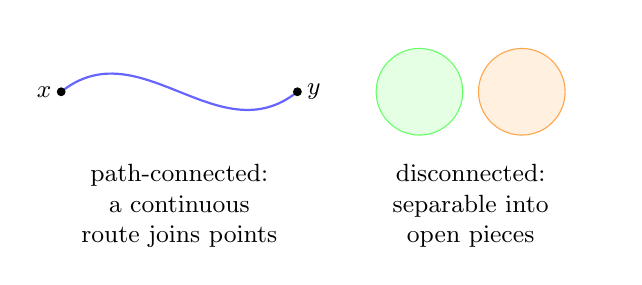
\begin{tikzpicture}[scale=1.0, every node/.style={font=\small}]
\draw[thick, blue!60] (0,0) .. controls (1,0.8) and (2,-0.8) .. (3,0);
\fill (0,0) circle (1.6pt) node[left] {$x$};
\fill (3,0) circle (1.6pt) node[right] {$y$};
\node[align=center, text width=3.4cm, anchor=north] at (1.5,-0.8) {path-connected:\\a continuous route joins points};
\begin{scope}[xshift=5cm]
\draw[fill=green!10, draw=green!60] (-0.45,0) circle (0.55);
\draw[fill=orange!12, draw=orange!70] (0.85,0) circle (0.55);
\node[align=center, text width=3.4cm, anchor=north] at (0.2,-0.8) {disconnected:\\separable into open pieces};
\end{scope}
\end{tikzpicture}
\end{center}

\begin{trapbox}
False intuition: connected means path-connected. Every path-connected space is
connected, but the converse can fail. Topology has examples where a space is
one piece in the open-set sense but still has no path between certain points.
\end{trapbox}

\begin{marginnotebox}
The theorem ``continuous images of connected spaces are connected'' is the
topological skeleton of the intermediate value theorem. The calculus statement
is familiar; topology shows the mechanism.
\end{marginnotebox}

\subsection{Compactness}

Compactness can be introduced through open covers.

\begin{definition}
Let $X$ be a topological space and $K\subseteq X$. An \emph{open cover} of $K$
is a collection of open sets $\{U_\alpha\}_{\alpha\in A}$ such that
\[
K\subseteq \bigcup_{\alpha\in A}U_\alpha.
\]
A \emph{finite subcover} is a finite subcollection
$U_{\alpha_1},\ldots,U_{\alpha_n}$ that still covers $K$.
\end{definition}

\begin{definition}
A set $K$ is \emph{compact} if every open cover of $K$ has a finite subcover.
\end{definition}

This definition is abstract but powerful. It says that whenever infinitely many
open sets are enough to cover $K$, finitely many were already enough.

\begin{intuitionbox}
Compactness is a finite-control principle. It lets you extract finite data from
an apparently infinite situation.
\end{intuitionbox}

\begin{center}
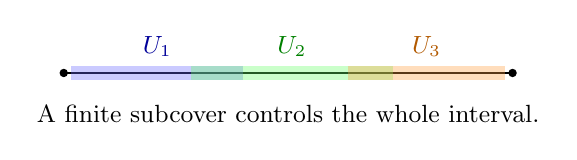
\begin{tikzpicture}[scale=0.95, every node/.style={font=\small}]
\draw[thick] (0,0) -- (6,0);
\foreach \x/\lab in {0/[0],6/[1]} {
  \fill (\x,0) circle (1.6pt);
}
\draw[blue!60, line width=5pt, opacity=0.35] (0.1,0) -- (2.4,0);
\draw[green!60, line width=5pt, opacity=0.35] (1.7,0) -- (4.4,0);
\draw[orange!75, line width=5pt, opacity=0.35] (3.8,0) -- (5.9,0);
\node[blue!60!black] at (1.25,0.35) {$U_1$};
\node[green!50!black] at (3.05,0.35) {$U_2$};
\node[orange!70!black] at (4.85,0.35) {$U_3$};
\node at (3,-0.55) {A finite subcover controls the whole interval.};
\end{tikzpicture}
\end{center}

This picture is deliberately too simple. A real open cover of $[0,1]$ may involve infinitely many open sets of wildly different sizes. Compactness says that if the cover works at all, finitely many of those open sets already do the job.

\begin{trapbox}
False intuition: compact just means closed and bounded. In $\R^n$, Heine-Borel says compact is equivalent to closed and bounded. In general topological spaces, that slogan can fail badly. The portable definition is the open-cover definition.
\end{trapbox}

\begin{example}
The interval $[0,1]$ is compact in $\R$. The interval $(0,1)$ is not compact.
The open cover
\[
\left\{(1/n,1):n=2,3,4,\ldots\right\}
\]
covers $(0,1)$ but no finite subcollection covers all of $(0,1)$.
\end{example}

\begin{theorem}
The continuous image of a compact space is compact.
\end{theorem}

\begin{proof}
Let $f:X\to Y$ be continuous and suppose $X$ is compact. Let
$\{V_\alpha\}_{\alpha\in A}$ be an open cover of $f(X)$ in $Y$. Then
$\{f^{-1}(V_\alpha)\}_{\alpha\in A}$ is an open cover of $X$. Since $X$ is
compact, there exist $\alpha_1,\ldots,\alpha_n$ such that
\[
X\subseteq f^{-1}(V_{\alpha_1})\cup\cdots\cup f^{-1}(V_{\alpha_n}).
\]
Applying $f$, we get
\[
f(X)\subseteq V_{\alpha_1}\cup\cdots\cup V_{\alpha_n}.
\]
Thus the original cover has a finite subcover. Therefore $f(X)$ is compact.
\end{proof}

Again, inverse images do the work. The proof pattern is central: pull a cover
back to the domain, use compactness there, push the finite result forward.

\begin{aestheticbox}
Compactness feels magical because it converts infinite information into finite
control. An arbitrary cover may contain infinitely many open sets, but compactness
says finitely many already suffice. This is why compactness powers existence
theorems throughout analysis and geometry.
\end{aestheticbox}

\begin{center}
\begin{tikzpicture}[scale=1.0, every node/.style={font=\small}]
\draw[thick] (0,0) -- (6,0);
\fill (0,0) circle (1.6pt);
\fill (6,0) circle (1.6pt);
\foreach \x/\w/\c in {0.1/1.0/sourceblue,0.75/0.8/targetgreen,1.35/1.4/quotientorange,2.6/0.9/sourceblue,3.2/1.6/targetgreen,4.5/1.2/quotientorange,5.25/0.7/sourceblue} {
  \draw[\c, line width=4pt, opacity=0.30] (\x,0.18) -- ++(\w,0);
}
\node at (3,-0.45) {many open sets cover the interval};
\draw[-{Latex}, thick] (3,-0.8) -- (3,-1.35);
\draw[thick] (0,-1.75) -- (6,-1.75);
\draw[sourceblue, line width=5pt, opacity=0.45] (0.1,-1.75) -- (1.1,-1.75);
\draw[quotientorange, line width=5pt, opacity=0.45] (1.35,-1.75) -- (2.75,-1.75);
\draw[targetgreen, line width=5pt, opacity=0.45] (3.2,-1.75) -- (4.8,-1.75);
\draw[quotientorange, line width=5pt, opacity=0.45] (4.5,-1.75) -- (5.7,-1.75);
\node at (3,-2.22) {compactness extracts finite control};
\end{tikzpicture}
\end{center}

\subsection{Bases}

Listing every open set can be inefficient. A basis gives building blocks.

\begin{definition}
A \emph{basis} for a topology on $X$ is a collection $\mathcal{B}$ of subsets
of $X$ such that:
\begin{enumerate}
\item for every $x\in X$, there is $B\in\mathcal{B}$ with $x\in B$,
\item if $x\in B_1\cap B_2$ with $B_1,B_2\in\mathcal{B}$, then there exists
$B_3\in\mathcal{B}$ such that $x\in B_3\subseteq B_1\cap B_2$.
\end{enumerate}
The open sets are unions of basis elements.
\end{definition}

\begin{example}
The open intervals $(a,b)$ form a basis for the usual topology on $\R$.
Open balls form a basis for the topology of any metric space.
\end{example}

The basis idea previews charts in differential geometry. A manifold is built
from coordinate neighborhoods that look like open subsets of $\R^n$.

\subsection{Product spaces}

If $X$ and $Y$ are spaces, their product $X\times Y$ should also be a space.
The product topology is generated by sets of the form $U\times V$, where $U$ is
open in $X$ and $V$ is open in $Y$.

\begin{example}
The usual topology on $\R^2$ is the product topology on $\R\times\R$. Open
rectangles form a basis, and open disks can be built from unions of rectangles.
\end{example}

Product spaces allow topology to model systems with several independent
coordinates. They also appear in algebraic geometry, differential geometry,
functional analysis, and probability.

\subsection{Quotient spaces}

Quotients identify points according to an equivalence relation.

\begin{definition}
Let $X$ be a topological space and let $\sim$ be an equivalence relation on
$X$. The quotient set $X/{\sim}$ is the set of equivalence classes. The
\emph{quotient topology} is defined by declaring $U\subseteq X/{\sim}$ open
if and only if its preimage under the quotient map $q:X\to X/{\sim}$ is open
in $X$.
\end{definition}

This definition mirrors the continuity definition. The quotient topology is the
topology that makes the quotient map continuous while preserving as much openness
as possible.

\begin{example}
If we take the interval $[0,1]$ and identify $0\sim 1$, the quotient space is a
circle. This is one rigorous way to build $S^1$ from an interval.
\end{example}

\begin{center}
\begin{tikzpicture}[scale=1.0, every node/.style={font=\small}]
\draw[thick] (0,0) -- (4,0);
\fill[red!70] (0,0) circle (2pt) node[below] {$0$};
\fill[red!70] (4,0) circle (2pt) node[below] {$1$};
\draw[-{Latex}, thick, bend left=45] (0,0.12) to node[above] {identify endpoints} (4,0.12);
\begin{scope}[xshift=6cm]
\draw[thick] (0,0) circle (0.85);
\fill[red!70] (0,0.85) circle (2pt);
\node at (0,-1.2) {$[0,1]/(0\sim1)\cong S^1$};
\end{scope}
\end{tikzpicture}
\end{center}

\begin{example}
If we take a square and identify opposite edges in the same direction, the
quotient space is a torus.
\end{example}

\begin{center}
\begin{tikzpicture}[scale=0.95, every node/.style={font=\small}]
\draw[thick] (0,0) rectangle (2.2,2.2);
\draw[-{Latex}, blue!70, thick] (0.35,2.2) -- (1.85,2.2);
\draw[-{Latex}, blue!70, thick] (0.35,0) -- (1.85,0);
\draw[-{Latex}, green!60!black, thick] (0,0.35) -- (0,1.85);
\draw[-{Latex}, green!60!black, thick] (2.2,0.35) -- (2.2,1.85);
\node at (1.1,-0.45) {identify matching edges};
\node at (4.3,1.1) {$\leadsto$ torus};
\draw[thick] (5.8,1.1) ellipse (1.0 and 0.45);
\draw[thick] (5.8,1.1) ellipse (0.42 and 0.95);
\node at (5.8,-0.45) {schematic};
\end{tikzpicture}
\end{center}

\begin{intuitionbox}
Quotient topology is controlled gluing. Algebra quotients forget differences;
topology quotients glue points while tracking which sets remain open.
\end{intuitionbox}

\begin{trapbox}
False intuition: quotient spaces are just ordinary subsets with renamed points.
Better intuition: quotienting changes the space. It can create loops, cones,
projective spaces, and strange identifications. The quotient topology is the
rulebook that keeps continuity honest after gluing.
\end{trapbox}

\begin{aestheticbox}
Quotients are beautiful because they make ``controlled forgetting'' precise.
You decide which distinctions no longer matter, then ask what structure survives
that decision.
\end{aestheticbox}

\subsection{Topology Visual Gallery: Deformation, Gluing, and Pathology}

Topology needs pictures, but it also teaches you not to trust pictures too
quickly. The right workflow is: let the picture suggest the idea, then let the
definition decide the truth.

\subsubsection*{Deformation intuition}

\begin{center}
\begin{tikzpicture}[scale=0.95, every node/.style={font=\small}]
\draw[thick, sourceblue] (0,0) circle (0.8);
\node at (0,-1.15) {circle};
\draw[-{Latex}, thick] (1.2,0) -- (2.2,0);
\draw[thick, sourceblue] (3.0,0) ellipse (1.1 and 0.55);
\node at (3.0,-1.15) {ellipse};
\draw[-{Latex}, thick] (4.4,0) -- (5.4,0);
\draw[thick, sourceblue] (6.2,0) .. controls (5.5,0.65) and (6.9,0.85) .. (7.15,0.15)
  .. controls (7.45,-0.55) and (5.75,-0.7) .. (6.2,0);
\node at (6.4,-1.15) {deformed loop};
\node[align=center, text width=8cm] at (3.4,-2.0) {Topological sameness permits stretching and bending, but not cutting or gluing.};
\end{tikzpicture}
\end{center}

\subsubsection*{Pathological warning}

Some spaces defeat ordinary drawing intuition. The topologist's sine curve is
the closure of
\[
y=\sin(1/x),\qquad 0<x\leq 1,
\]
together with a limiting vertical segment at $x=0$.

\begin{center}
\begin{tikzpicture}[scale=1.0, every node/.style={font=\small}]
\draw[->] (-0.2,0) -- (5.2,0) node[right] {$x$};
\draw[->] (0,-1.3) -- (0,1.3) node[above] {$y$};
\draw[trapred, thick] (0,-1) -- (0,1);
\draw[sourceblue, thick, samples=220, domain=0.16:4.8, smooth, variable=\t]
  plot ({\t},{sin(4.8*180/\t)});
\node[trapred] at (0.75,1.05) {limit segment};
\node[align=center, text width=7.2cm] at (2.7,-1.75) {This standard example is connected but not path-connected. It corrects the naive idea that ``one piece'' always means ``walkable between any two points.''};
\end{tikzpicture}
\end{center}

\begin{trapbox}
False intuition: every connected subset of the plane behaves like a familiar
region. Pathological examples are why topology insists on definitions instead
of only visual confidence.
\end{trapbox}

\subsubsection*{Manifold charts as topology plus coordinates}

\begin{center}
\begin{tikzpicture}[scale=1.0, every node/.style={font=\small}]
\draw[thick, fill=sourceblue!8, draw=sourceblue] (0,0) circle (1.1);
\draw[structurepurple, thick, fill=structurepurple!12] (-0.25,0.25) circle (0.45);
\node[sourceblue] at (0,-1.4) {space $M$};
\draw[-{Latex}, thick] (1.35,0.35) -- node[above] {chart $\varphi$} (3.2,0.75);
\draw[thick, fill=targetgreen!8, draw=targetgreen] (3.6,0) rectangle (5.4,1.5);
\draw[structurepurple, thick, fill=structurepurple!12] (4.45,0.75) ellipse (0.55 and 0.35);
\node[targetgreen] at (4.5,-0.35) {open set in $\R^n$};
\end{tikzpicture}
\end{center}

This foreshadows differential geometry. Topology supplies open sets and local
patches; calculus enters through coordinate maps.

\begin{aestheticbox}
Topology is powerful because it keeps only enough structure to discuss
continuity. By forgetting measurement, it lets deeper invariants become visible.
\end{aestheticbox}

\subsection{Topological invariants}

A topological invariant is a property preserved by homeomorphism. If two spaces
have different values of an invariant, they cannot be homeomorphic.

Examples of basic invariants include:

\begin{itemize}
\item number of connected components,
\item compactness,
\item connectedness,
\item path-connectedness,
\item whether removing a point disconnects the space,
\item fundamental group, in later algebraic topology.
\end{itemize}

\begin{example}
The spaces $(0,1)$ and $[0,1]$ are not homeomorphic. One reason is compactness:
$[0,1]$ is compact, while $(0,1)$ is not.
\end{example}

\begin{example}
The spaces $\R$ and $\R^2$ are not homeomorphic, though proving this rigorously
requires more topology. A suggestive invariant is what happens when a point is
removed: $\R\setminus\{0\}$ is disconnected, but $\R^2\setminus\{(0,0)\}$ is
connected.
\end{example}

Invariants are proof tools. To show two spaces are the same, build a
homeomorphism. To show they are different, find an invariant that separates
them.

\subsection{Path-connectedness}

Connectedness says a space cannot be separated into two disjoint open pieces.
Path-connectedness is more concrete: any two points can be joined by a
continuous path.

\begin{definition}
A space $X$ is \emph{path-connected} if for every $x,y\in X$, there exists a
continuous function
\[
\gamma:[0,1]\to X
\]
such that $\gamma(0)=x$ and $\gamma(1)=y$.
\end{definition}

\begin{theorem}
Every path-connected space is connected.
\end{theorem}

\begin{proof}
Suppose $X$ is path-connected and disconnected. Then $X=U\cup V$ where $U$ and
$V$ are nonempty disjoint open sets. Choose $u\in U$ and $v\in V$. Since $X$ is
path-connected, there is a continuous path $\gamma:[0,1]\to X$ with
$\gamma(0)=u$ and $\gamma(1)=v$.

The sets $\gamma^{-1}(U)$ and $\gamma^{-1}(V)$ form a separation of $[0,1]$,
contradicting the connectedness of the interval. Therefore $X$ is connected.
\end{proof}

The converse is not always true, though it is true for many familiar spaces such
as intervals and open connected subsets of $\R^n$ with suitable hypotheses.

\subsection{A first glimpse of algebraic topology}

Algebraic topology assigns algebraic objects to topological spaces. The simplest
idea to preview is the fundamental group, which records loops up to continuous
deformation.

\begin{definition}
A \emph{loop} in a space $X$ based at $x_0$ is a continuous map
\[
\gamma:[0,1]\to X
\]
such that $\gamma(0)=\gamma(1)=x_0$.
\end{definition}

Loops can be concatenated: travel around one loop, then another. Up to a
suitable equivalence relation called homotopy, loop classes form a group called
the fundamental group. The full construction belongs later, but the intuition is
useful now.

\begin{example}
In the plane $\R^2$, every loop can be continuously shrunk to a point. Around a
punctured plane $\R^2\setminus\{0\}$, a loop may wind around the missing point.
The winding number is algebraic information extracted from topology.
\end{example}

\begin{focusbox}
Algebraic topology continues the theme of this reader: use maps and equivalence
relations to convert geometric questions into algebraic ones.
\end{focusbox}

\subsection{Common proof habits in topology}

Topology proofs often feel clean once definitions are unpacked. Common moves
include:

\begin{itemize}
\item prove continuity by pulling back open sets,
\item prove non-continuity by finding one open set whose preimage is not open,
\item prove compactness by starting with an arbitrary open cover,
\item prove connectedness by assuming a separation and deriving a contradiction,
\item use bases to reduce ``all open sets'' to simpler building blocks,
\item use quotient maps by checking preimages in the original space.
\end{itemize}

\begin{trapbox}
Do not rely too heavily on pictures. Pictures are valuable, but topological
proofs are usually about open sets, maps, covers, and equivalence relations.
When a picture suggests a claim, translate it into one of those languages.
\end{trapbox}

\subsection{Applications of topology}

Topology supports:

\begin{itemize}
\item qualitative analysis of dynamical systems,
\item data analysis through persistent homology,
\item compactness methods in analysis,
\item manifolds in geometry and physics,
\item fixed point theorems,
\item configuration spaces in robotics,
\item continuity arguments in economics and optimization,
\item algebraic topology and invariants of spaces.
\end{itemize}

One reason topology is so portable is that it uses few assumptions. Whenever a
problem has continuity but not necessarily a convenient formula or metric,
topology may still apply.

\subsection{Proof lab: compactness and closed subsets}

Compactness becomes more useful when combined with ordinary set operations.

\begin{theorem}
If $K$ is compact and $F\subseteq K$ is closed, then $F$ is compact.
\end{theorem}

\begin{proof}
Let $\{U_\alpha\}_{\alpha\in A}$ be an open cover of $F$. Since $F$ is closed
in $K$, the complement $K\setminus F$ is open in $K$. Then the collection
\[
\{U_\alpha\}_{\alpha\in A}\cup\{K\setminus F\}
\]
is an open cover of $K$. Since $K$ is compact, finitely many of these sets cover
$K$. Removing $K\setminus F$ if it appears, the remaining finitely many
$U_\alpha$ cover $F$. Therefore $F$ is compact.
\end{proof}

This proof is a model for working with open covers. You start with an arbitrary
cover of the smaller set, add one extra open set to cover the rest of the compact
space, use compactness, and then restrict back to the original set.

\begin{labbox}
Use the theorem to prove that any closed interval $[a,b]$ is compact once you
know that a larger interval $[-M,M]$ is compact and contains $[a,b]$.
\end{labbox}

\subsection{Counterexample lab: topology is context}

Topology trains you to produce examples that separate similar-looking ideas.

\begin{example}
A compact space need not be finite. The interval $[0,1]$ is compact and
infinite.
\end{example}

\begin{example}
A connected space need not be path-connected. The topologist's sine curve is a
standard example, though its full analysis is beyond this preview.
\end{example}

\begin{example}
A set can be both open and closed. In any topological space $X$, both
$\emptyset$ and $X$ are clopen. In a disconnected space, nontrivial clopen sets
also exist.
\end{example}

\begin{example}
A topology can be too coarse to distinguish points. In the indiscrete topology
on a set with at least two points, no two distinct points can be separated by
disjoint open sets.
\end{example}

\begin{focusbox}
Topology is a field where examples do a lot of teaching. When two definitions
feel similar, look for a space where they come apart.
\end{focusbox}

\subsection{Exercises for topology}

\begin{exercise}
Let $X=\{a,b,c\}$. Decide whether
\[
\mathcal{T}=\{\emptyset,X,\{a\},\{a,b\}\}
\]
is a topology on $X$.
\end{exercise}

\begin{exercise}
Prove that the union of any collection of open sets in a metric space is open.
\end{exercise}

\begin{exercise}
Prove that the finite intersection of open sets in a metric space is open.
Where does finiteness enter?
\end{exercise}

\begin{exercise}
Let $f:\R\to\R$ be given by $f(x)=x^2$. Using the topological definition of
continuity, explain why it is enough to know the usual epsilon-delta theorem
from analysis.
\end{exercise}

\begin{exercise}
Give an open cover of $(0,1)$ with no finite subcover.
\end{exercise}

\begin{exercise}
Explain why a constant map $f:X\to Y$ is continuous for every pair of
topological spaces $X$ and $Y$.
\end{exercise}

\begin{exercise}
In the subspace $[0,1]\subseteq\R$, decide whether each set is open:
$[0,1/2)$, $(1/3,2/3)$, $\{0\}$, and $[0,1]$.
\end{exercise}

\begin{exercise}
Prove that every metric space is Hausdorff.
\end{exercise}

\begin{exercise}
Show that if $X$ is path-connected and $f:X\to Y$ is continuous, then $f(X)$
is path-connected.
\end{exercise}

\begin{walkbox}
What properties of an object survive stretching, bending, or reparameterizing?
Which properties require measurement? Sort familiar facts into topological and
geometric categories.
\end{walkbox}

\section{Preview Chapter: Differential Geometry}

Differential geometry studies spaces that are curved but locally accessible by
calculus. The central objects are manifolds: spaces that may not be linear or
flat globally, but near each point resemble ordinary Euclidean space.

This field connects early proof ideas to a rich geometric setting. Definitions
matter intensely. A curve is not just a drawn line; it is often a smooth map
from an interval. A tangent vector is not just an arrow in a picture; it can be
defined as a velocity, a derivation, or an equivalence class of curves. A
manifold is not just a surface in $\R^3$; it is a space with compatible local
coordinate systems.

\begin{focusbox}
Differential geometry is calculus plus topology plus linear algebra, organized
so that local computations say something about global shape.
\end{focusbox}

\subsection{Historical motivation}

Classical geometry studied lines, circles, conics, and surfaces. Calculus made
it possible to study curves and surfaces through derivatives. Gauss showed that
curvature could be intrinsic: a surface could have geometry detectable by beings
living on it, without reference to the surrounding three-dimensional space.

Riemann then generalized geometry by allowing spaces of any dimension with a
notion of length that could vary from point to point. This became essential for
modern physics, especially general relativity, where gravity is modeled as
curvature of spacetime.

\begin{historybox}
Gauss's \emph{Theorema Egregium}, the ``remarkable theorem,'' showed that
Gaussian curvature is intrinsic. You can bend a sheet of paper into a cylinder
without stretching it, and its intrinsic curvature remains zero. A sphere cannot
be flattened without distortion because its intrinsic curvature is positive.
\end{historybox}

\subsection{Curves as maps}

A curve is best understood as a function, not merely as a subset.

\begin{definition}
A \emph{parametrized curve} in $\R^n$ is a function
\[
\gamma:I\to\R^n
\]
where $I\subseteq\R$ is an interval. The curve is \emph{smooth} if all component
functions are differentiable as often as needed.
\end{definition}

\begin{example}
The unit circle can be parametrized by
\[
\gamma(t)=(\cos t,\sin t),\qquad 0\leq t<2\pi.
\]
The image is the circle, but the map also contains information about speed and
direction.
\end{example}

The derivative of a curve is its velocity:
\[
\gamma'(t)=\left(\gamma_1'(t),\ldots,\gamma_n'(t)\right).
\]

\begin{example}
For $\gamma(t)=(\cos t,\sin t)$,
\[
\gamma'(t)=(-\sin t,\cos t).
\]
At $t=0$, the point is $(1,0)$ and the velocity is $(0,1)$.
\end{example}

\begin{trapbox}
Do not confuse a curve's image with the curve as a parametrized map. The maps
$\gamma(t)=(\cos t,\sin t)$ and $\eta(t)=(\cos 2t,\sin 2t)$ trace the same
circle at different speeds.
\end{trapbox}

\subsection{Arc length}

For a smooth curve $\gamma:[a,b]\to\R^n$, the length is
\[
L(\gamma)=\int_a^b \|\gamma'(t)\|\,dt.
\]
This formula is familiar from calculus, but differential geometry asks how it
behaves under reparametrization.

\begin{example}
For the unit circle parametrization $\gamma(t)=(\cos t,\sin t)$ on
$[0,2\pi]$, we have
\[
\|\gamma'(t)\|=\sqrt{(-\sin t)^2+(\cos t)^2}=1.
\]
Therefore
\[
L(\gamma)=\int_0^{2\pi}1\,dt=2\pi.
\]
\end{example}

If the same circle is traced twice as fast, the speed doubles but the time
interval halves for one trip. The length remains $2\pi$. This is an early sign
of geometric invariance: a quantity should not depend on an arbitrary coordinate
choice.

\subsection{Surfaces and local coordinates}

A surface in $\R^3$ can often be described by a parametrization
\[
X:U\subseteq\R^2\to\R^3.
\]
For example, the sphere of radius $1$ can be parametrized, away from coordinate
singularities, by
\[
X(\theta,\phi)=(\sin\phi\cos\theta,\sin\phi\sin\theta,\cos\phi).
\]

The parameters $(\theta,\phi)$ are coordinates. They are useful, but they are
not the surface itself. At the poles, these spherical coordinates behave badly:
different values of $\theta$ describe the same point. This motivates the
manifold idea, where one uses many coordinate charts rather than demanding one
global coordinate system.

\begin{intuitionbox}
A chart is a local coordinate API. It lets you do Euclidean calculations near a
point, but it may not cover the whole space cleanly.
\end{intuitionbox}

\subsection{Manifolds}

The topological starting point is that each small region should look like an
open subset of $\R^n$.

\begin{definition}
An \emph{$n$-dimensional topological manifold} is a topological space $M$ such
that every point $p\in M$ has a neighborhood $U$ homeomorphic to an open subset
of $\R^n$. The pair $(U,\varphi)$, where
\[
\varphi:U\to \varphi(U)\subseteq\R^n
\]
is a homeomorphism, is called a \emph{chart}.
\end{definition}

To do calculus, the charts must be compatible smoothly.

\begin{definition}
A \emph{smooth manifold} is a manifold with charts whose transition maps are
smooth. If $(U,\varphi)$ and $(V,\psi)$ overlap, the transition map is
\[
\psi\circ\varphi^{-1}:\varphi(U\cap V)\to\psi(U\cap V).
\]
\end{definition}

This definition is a direct meeting point of topology, functions, and calculus.
Charts are homeomorphisms. Transition maps are compositions. Smoothness is
checked in Euclidean coordinates.

\begin{example}
The circle $S^1$ is a one-dimensional manifold. Near any point, a small arc of
the circle looks like an open interval.
\end{example}

\begin{example}
The sphere $S^2$ is a two-dimensional manifold. No single chart covers it
without distortion or singularity, but stereographic projection gives charts
from the sphere minus one point to $\R^2$.
\end{example}

\begin{trapbox}
An $n$-dimensional manifold need not live inside $\R^n$. The circle is
one-dimensional but is usually drawn in $\R^2$. The sphere is two-dimensional
but is usually drawn in $\R^3$.
\end{trapbox}

\subsection{Tangent spaces}

At each point of a smooth manifold, there is a vector space of tangent
directions.

For a surface sitting in $\R^3$, the tangent plane can be visualized as the best
linear approximation to the surface at a point. For an abstract manifold, we
need a definition that does not depend on an ambient space.

\begin{definition}
Let $M$ be a smooth manifold and $p\in M$. A tangent vector at $p$ can be viewed
as an equivalence class of smooth curves $\gamma:(-\eps,\eps)\to M$ with
$\gamma(0)=p$, where two curves are equivalent if their coordinate
representations have the same derivative at $0$ in some, and hence any, chart.
The set of tangent vectors at $p$ is called the \emph{tangent space} $T_pM$.
\end{definition}

This definition looks technical because it protects an intuitive idea from
coordinate dependence. A tangent vector should be a direction through $p$, not
an artifact of one chart.

\begin{example}
For $M=\R^n$, the tangent space $T_p\R^n$ can be identified with $\R^n$ itself.
At every point of Euclidean space, the possible velocity vectors are ordinary
vectors.
\end{example}

\begin{example}
For the unit sphere $S^2\subseteq\R^3$, the tangent space at $p\in S^2$ is
\[
T_pS^2=\{v\in\R^3:v\cdot p=0\}.
\]
This is the plane through the origin perpendicular to $p$, translated in the
usual picture to touch the sphere at $p$.
\end{example}

\subsection{Implicit surfaces}

Many surfaces are not given first by parametrizations. They are given as level
sets of functions.

\begin{definition}
Let $F:\R^3\to\R$ be smooth. A set
\[
S=\{(x,y,z)\in\R^3:F(x,y,z)=c\}
\]
is a \emph{level surface}. If $\nabla F(p)\neq 0$ at a point $p\in S$, then
near $p$ the set $S$ is a smooth surface.
\end{definition}

This is an informal version of the implicit function theorem. It says that a
single equation in three variables usually cuts out a two-dimensional surface,
provided the gradient does not vanish.

\begin{example}
For the sphere,
\[
F(x,y,z)=x^2+y^2+z^2.
\]
The unit sphere is $F^{-1}(1)$. Since
\[
\nabla F=(2x,2y,2z),
\]
the gradient is nonzero at every point of the unit sphere. Therefore the sphere
is a smooth surface.
\end{example}

The tangent plane to a level surface has a simple description:
\[
T_pS=\{v\in\R^3:\nabla F(p)\cdot v=0\}.
\]
This is the same calculation used earlier for the circle.

\begin{trapbox}
If the gradient vanishes, the level set may still be smooth, but the simple
test no longer proves it. A zero gradient is a warning that singular behavior
may be present.
\end{trapbox}

\subsection{Differentials}

A smooth map between manifolds has a derivative at each point, called its
differential or pushforward.

\begin{definition}
Let $F:M\to N$ be a smooth map and let $p\in M$. The \emph{differential}
\[
dF_p:T_pM\to T_{F(p)}N
\]
sends the velocity of a curve $\gamma$ through $p$ to the velocity of the curve
$F\circ\gamma$ through $F(p)$.
\end{definition}

In Euclidean space, this is the Jacobian matrix. On manifolds, the same idea is
written in coordinate-independent language.

\begin{example}
Let $F:\R^2\to\R$ be $F(x,y)=x^2+y^2$. At $(a,b)$, the differential is the
linear map
\[
dF_{(a,b)}(u,v)=2au+2bv.
\]
This is the directional rate of change of $F$ at $(a,b)$ in direction $(u,v)$.
\end{example}

\begin{focusbox}
Differential geometry repeatedly replaces nonlinear objects by linear
approximations at a point. Tangent spaces are where that linearization lives.
\end{focusbox}

\subsection{Vector fields}

A vector field assigns a tangent vector to each point.

\begin{definition}
A \emph{vector field} on a smooth manifold $M$ assigns to each $p\in M$ a
vector $X_p\in T_pM$, smoothly in $p$.
\end{definition}

On $\R^2$, a vector field can be written
\[
X(x,y)=P(x,y)\frac{\partial}{\partial x}+Q(x,y)\frac{\partial}{\partial y}.
\]
You have seen vector fields in differential equations and physics: velocity
fields, force fields, gradient fields, and flow fields.

\begin{example}
The vector field
\[
X(x,y)=(-y,x)
\]
on $\R^2$ rotates around the origin. Its integral curves are circles centered
at the origin.
\end{example}

The language of vector fields turns differential equations into geometry. A
solution curve is a curve whose velocity at each point matches the vector field.

\subsection{Flows}

A vector field often generates a flow: a family of transformations describing
where each point moves after time $t$.

\begin{definition}
Given a vector field $X$ on a manifold $M$, an \emph{integral curve} through
$p\in M$ is a smooth curve $\gamma:I\to M$ such that
\[
\gamma(0)=p,\qquad \gamma'(t)=X_{\gamma(t)}.
\]
\end{definition}

In Euclidean language, this is an ordinary differential equation. Differential
geometry interprets it as motion on a manifold.

\begin{example}
For $X(x,y)=(-y,x)$ on $\R^2$, the curve
\[
\gamma(t)=(\cos t,\sin t)
\]
is an integral curve through $(1,0)$ because
\[
\gamma'(t)=(-\sin t,\cos t)=X(\gamma(t)).
\]
\end{example}

Flows connect differential geometry with dynamical systems. The local existence
and uniqueness theorem for ordinary differential equations becomes a theorem
about vector fields producing local motion on manifolds.

\subsection{Lie groups}

Some spaces are both manifolds and groups. These are Lie groups.

\begin{definition}
A \emph{Lie group} is a group $G$ that is also a smooth manifold, such that the
multiplication map
\[
G\times G\to G,\qquad (g,h)\mapsto gh
\]
and inverse map
\[
G\to G,\qquad g\mapsto g^{-1}
\]
are smooth.
\end{definition}

\begin{example}
The circle
\[
S^1=\{z\in\C:|z|=1\}
\]
is a Lie group under complex multiplication. It is also a one-dimensional
manifold.
\end{example}

\begin{example}
The group $GL(n,\R)$ of invertible $n\times n$ real matrices is a Lie group.
It is an open subset of $\R^{n^2}$ because invertibility is the condition
$\det(A)\neq 0$.
\end{example}

Lie groups show how algebra and geometry combine. Their tangent spaces at the
identity become Lie algebras, which encode infinitesimal symmetry.

\begin{intuitionbox}
A Lie group is a smooth family of symmetries. Group theory describes how
symmetries compose; differential geometry describes how they vary continuously.
\end{intuitionbox}

\subsection{Differential forms}

Differential forms are objects that can be integrated over curves, surfaces,
and higher-dimensional manifolds. A one-form eats a vector and returns a number.

\begin{definition}
On $\R^n$, a \emph{one-form} is an expression
\[
\omega=f_1\,dx_1+\cdots+f_n\,dx_n
\]
where the $f_i$ are smooth functions. At each point, $\omega$ is a linear
function on tangent vectors.
\end{definition}

\begin{example}
On $\R^2$, let
\[
\omega=y\,dx+x\,dy.
\]
If $v=(u,w)$ is a tangent vector at $(x,y)$, then
\[
\omega(v)=yu+xw.
\]
\end{example}

Forms are the natural language of integration on manifolds. They lead to
Stokes' theorem, which unifies the fundamental theorem of calculus, Green's
theorem, the divergence theorem, and Stokes' theorem from vector calculus.

\begin{theorem}[Stokes' theorem, preview]
For a suitable differential form $\omega$ on a suitable oriented manifold $M$,
\[
\int_M d\omega=\int_{\partial M}\omega.
\]
\end{theorem}

This statement is too compressed for a first proof here, but its message is
important: the integral of a derivative over a region equals the integral of the
original object over the boundary.

\subsection{Metrics and curvature}

A Riemannian metric gives a smoothly varying inner product on tangent spaces.

\begin{definition}
A \emph{Riemannian metric} on a smooth manifold $M$ assigns to each point
$p\in M$ an inner product
\[
g_p:T_pM\times T_pM\to\R
\]
that varies smoothly with $p$.
\end{definition}

With a metric, one can measure lengths of tangent vectors, angles between
vectors, lengths of curves, areas, volumes, gradients, and curvature.

\begin{example}
The usual dot product on $\R^n$ is a Riemannian metric. In coordinates,
\[
g_p(v,w)=v\cdot w.
\]
\end{example}

Curvature measures how a geometric space departs from being flat. For a curve,
curvature measures how quickly the tangent direction changes. For a surface,
Gaussian curvature captures intrinsic bending.

\begin{example}
A plane has Gaussian curvature $0$. A sphere of radius $R$ has constant
positive Gaussian curvature $1/R^2$. A saddle surface has negative curvature
near the saddle point.
\end{example}

\begin{intuitionbox}
Curvature is not merely how something looks from outside. Intrinsic curvature
can be detected by measurements made inside the space, such as angle sums of
triangles or how circles' circumferences compare to $2\pi r$.
\end{intuitionbox}

\subsection{Geodesics}

Geodesics generalize straight lines. They are locally length-minimizing paths,
or equivalently paths that move straight according to the geometry of the
manifold.

\begin{example}
On the plane, geodesics are straight lines. On the sphere, geodesics are great
circles, such as the equator and lines of longitude.
\end{example}

This has practical consequences. Airplane routes drawn on a flat map may look
curved, but on the sphere the shortest routes follow great circles.

\subsection{Covariant derivatives, gently}

In ordinary Euclidean space, vectors at different points can be compared
directly. On a curved manifold, tangent vectors at different points live in
different tangent spaces. To differentiate vector fields, one needs a rule for
comparing nearby tangent spaces.

That rule is called a connection. The most important connection in Riemannian
geometry is the Levi-Civita connection, determined by the metric.

\begin{definition}
Informally, a \emph{covariant derivative} $\nabla_XY$ measures the rate of
change of a vector field $Y$ in the direction of a vector field $X$, while
respecting the manifold's geometry.
\end{definition}

This is too advanced for full formal development here, but the reason it exists
is beginner-friendly: the derivative of a vector field should again be geometric,
not an artifact of coordinates or an ambient space.

\begin{example}
On a sphere, a tangent vector can be moved along a curve while staying tangent
and changing as little as possible. This process is called parallel transport.
Moving around a closed loop may return the vector rotated. That failure to
return unchanged is a sign of curvature.
\end{example}

\subsection{Orientation}

Orientation is the structure needed to make consistent choices of positive
direction or positive volume.

\begin{example}
The real line has two orientations: left-to-right and right-to-left. The plane
has clockwise versus counterclockwise orientation. A sphere is orientable.
\end{example}

Some manifolds are not orientable. The standard beginner example is the Mobius
strip, which has only one side. If you move a small oriented frame around the
strip and return to the starting point, the orientation has flipped.

Orientation matters for integration. Stokes' theorem requires compatible
orientations on a manifold and its boundary.

\begin{trapbox}
Orientability is not the same as having a preferred orientation. A sphere is
orientable, but you still must choose which orientation to use.
\end{trapbox}

\subsection{Common proof habits in differential geometry}

Differential geometry proofs often have two layers: a coordinate calculation
and an argument that the result is independent of coordinates. Common moves
include:

\begin{itemize}
\item choose a chart near a point,
\item compute using ordinary calculus in coordinates,
\item check that the result does not depend on the chart,
\item reduce a manifold claim locally to a Euclidean claim,
\item use linear algebra on tangent spaces,
\item track how objects transform under change of coordinates.
\end{itemize}

\begin{trapbox}
Do not mistake coordinates for geometry. Coordinates are tools for computation.
The geometric object should make sense after changing coordinates.
\end{trapbox}

\subsection{Applications of differential geometry}

Differential geometry supports:

\begin{itemize}
\item general relativity and spacetime geometry,
\item robotics and configuration spaces,
\item computer graphics and surface processing,
\item optimization on manifolds,
\item mechanics and control theory,
\item gauge theory and modern physics,
\item shape analysis and geometric data processing.
\end{itemize}

For a software engineer, one accessible application is optimization on curved
spaces. If parameters are constrained to lie on a sphere, a rotation group, or a
space of positive definite matrices, ordinary Euclidean gradient descent may
leave the valid space. Riemannian optimization adapts gradient methods to the
manifold.

\subsection{Proof lab: coordinate changes on a curve}

A simple place to see coordinate dependence is a reparametrized curve. Let
\[
\gamma(t)=(\cos t,\sin t)
\]
and let
\[
\eta(s)=\gamma(2s)=(\cos 2s,\sin 2s).
\]
These curves have the same image if the parameter intervals are chosen
appropriately, but their velocities differ:
\[
\gamma'(t)=(-\sin t,\cos t),
\qquad
\eta'(s)=(-2\sin 2s,2\cos 2s).
\]
The speed of $\eta$ is twice the speed of $\gamma$.

The chain rule explains this:
\[
\eta'(s)=\gamma'(2s)\cdot 2.
\]
Thus velocity depends on parametrization, while the geometric trace does not.
Arc length remains invariant when the reparametrization is handled correctly.

\begin{labbox}
Let $\gamma(t)=(t,t^2)$ and $\eta(s)=\gamma(s^3)$. Compute $\eta'(s)$ using the
chain rule, then directly from the formula for $\eta(s)$.
\end{labbox}

\subsection{Geometry trap lab: embedded versus intrinsic}

A surface may be studied as a subset of Euclidean space, or intrinsically as a
space in its own right. Both views are useful, but they are not the same.

\begin{example}
A cylinder in $\R^3$ looks curved from outside, but intrinsically it is flat:
locally it has the same geometry as a plane. This is why a sheet of paper can
be rolled into a cylinder without stretching.
\end{example}

\begin{example}
A sphere has positive intrinsic curvature. No flat map of the Earth can preserve
all distances and angles globally.
\end{example}

\begin{trapbox}
Do not assume every visual bend is intrinsic curvature. Bending without
stretching can change extrinsic appearance while preserving intrinsic geometry.
\end{trapbox}

This distinction matters in applications. A robot arm's configuration space may
be a curved manifold because of constraints, even if it is described using many
ambient coordinates. The intrinsic geometry records the legal motions, not the
surrounding coordinate bookkeeping.

\subsection{Beginner worked example: tangent line to a circle}

Let $S^1=\{(x,y)\in\R^2:x^2+y^2=1\}$. At a point $p=(a,b)\in S^1$, the tangent
line should consist of vectors $v=(u,w)$ satisfying
\[
au+bw=0.
\]

Why? Let $\gamma(t)=(x(t),y(t))$ be a curve on the circle with $\gamma(0)=p$.
Since the curve stays on the circle,
\[
x(t)^2+y(t)^2=1
\]
for all $t$. Differentiate at $t=0$:
\[
2x(0)x'(0)+2y(0)y'(0)=0.
\]
Thus
\[
a u+b w=0
\]
where $v=\gamma'(0)=(u,w)$. The tangent vector is perpendicular to the radius.

\begin{labbox}
Use the same method to find the tangent plane to the sphere
\[
x^2+y^2+z^2=1
\]
at a point $(a,b,c)$ on the sphere.
\end{labbox}

\subsection{Exercises for differential geometry}

\begin{exercise}
Compute the velocity and speed of the curve
\[
\gamma(t)=(t,t^2)
\]
at time $t=1$.
\end{exercise}

\begin{exercise}
Find the length of the curve $\gamma(t)=(3\cos t,3\sin t)$ for
$0\leq t\leq 2\pi$.
\end{exercise}

\begin{exercise}
Explain why the circle $S^1$ is locally like $\R$ but not globally homeomorphic
to $\R$.
\end{exercise}

\begin{exercise}
Let $F:\R^2\to\R^2$ be $F(x,y)=(x^2-y^2,2xy)$. Compute the Jacobian matrix and
interpret it as $dF_{(a,b)}$.
\end{exercise}

\begin{exercise}
For the sphere $S^2$, verify that $T_pS^2=\{v:v\cdot p=0\}$ gives a
two-dimensional vector space for every $p\in S^2$.
\end{exercise}

\begin{exercise}
Let $F(x,y,z)=x^2+y^2-z$. Find the tangent plane to the level surface
$F=0$ at $(1,1,2)$.
\end{exercise}

\begin{exercise}
Show that $S^1$ is closed under complex multiplication and inverses. Then
explain why it is reasonable to call it a group of rotations.
\end{exercise}

\begin{exercise}
For the vector field $X(x,y)=(1,0)$ on $\R^2$, describe the integral curve
through an arbitrary point $(a,b)$.
\end{exercise}

\begin{walkbox}
Think about a map of the Earth. Where do coordinates help? Where do they break
down? What information belongs to the Earth itself rather than to the map?
\end{walkbox}

\section{Preview Chapter: Algebraic Geometry}

Algebraic geometry studies shapes defined by polynomial equations. The basic
idea is simple:
\[
\text{polynomial equations} \quad \longleftrightarrow \quad \text{geometric sets}.
\]
But this simple bridge becomes one of the deepest areas of mathematics because
polynomials carry both algebraic structure and geometric meaning.

At a beginner level, algebraic geometry should not be introduced as a wall of
schemes. It should begin with concrete equations: lines, circles, parabolas,
intersections, and solution sets. Then the algebraic language of rings and
ideals explains how equations organize geometry.

\begin{focusbox}
Algebraic geometry begins with a friendly question: what shape is described by
these polynomial equations? The mature subject asks the reverse question too:
what algebraic object records the functions on this shape?
\end{focusbox}

\subsection{Historical motivation}

Classical analytic geometry, associated with Descartes and Fermat, connected
equations with curves. A line could be written as $ax+by=c$. A circle could be
written as $x^2+y^2=r^2$. Geometry became algebraic.

Later, mathematicians studied higher-degree curves, intersections, singularities,
and solutions over different number systems. Algebraic geometry grew from this
interaction. It now reaches number theory, topology, representation theory,
cryptography, and mathematical physics.

\begin{historybox}
The phrase ``algebraic geometry'' reflects a two-way translation. Algebra gives
equations. Geometry gives shapes. Major advances came from learning that neither
side alone tells the whole story.
\end{historybox}

\subsection{Affine space}

The simplest setting is affine space.

\begin{definition}
Let $k$ be a field. The affine $n$-space over $k$ is
\[
\mathbb{A}^n_k=k^n.
\]
Its points are ordered $n$-tuples $(a_1,\ldots,a_n)$ with coordinates in $k$.
\end{definition}

When $k=\R$, $\mathbb{A}^2_\R$ is the usual coordinate plane. When $k=\C$, it is
the complex plane squared, which has real dimension four. When $k$ is a finite
field, affine space is a finite set of points.

The field matters. The equation
\[
x^2+1=0
\]
has no solution in $\R$ but has two solutions in $\C$. Algebraic geometry is
very sensitive to the choice of ground field.

\subsection{Affine varieties}

\begin{definition}
Let $k$ be a field and let $S\subseteq k[x_1,\ldots,x_n]$ be a set of
polynomials. The \emph{zero set} of $S$ is
\[
V(S)=\{a\in k^n:f(a)=0\text{ for every }f\in S\}.
\]
An \emph{affine algebraic set} is a subset of $k^n$ of the form $V(S)$.
\end{definition}

Some texts reserve the word \emph{variety} for irreducible algebraic sets. In a
beginner preview, it is common to use ``variety'' informally for a polynomial
zero set, but you should know that conventions vary.

\begin{example}
In $\R^2$, the polynomial $f(x,y)=y-x^2$ defines the parabola
\[
V(y-x^2)=\{(x,y)\in\R^2:y=x^2\}.
\]
\end{example}

\begin{example}
The polynomial $x^2+y^2-1$ defines the unit circle in $\R^2$:
\[
V(x^2+y^2-1)=\{(x,y):x^2+y^2=1\}.
\]
\end{example}

\begin{example}
The pair of equations
\[
y-x^2=0,\qquad y-1=0
\]
defines the intersection of the parabola $y=x^2$ with the line $y=1$. The
solutions over $\R$ are $(-1,1)$ and $(1,1)$.
\end{example}

\begin{intuitionbox}
One polynomial gives a hypersurface. Several polynomials give an intersection
of hypersurfaces. Algebraic geometry studies those intersections using the
algebra of the polynomials.
\end{intuitionbox}

\subsection{The algebra of equations}

If two equations vanish on a set, then many combinations vanish too. Suppose
$f(a)=0$ and $g(a)=0$. Then
\[
(f+g)(a)=0,\qquad (hf)(a)=0
\]
for any polynomial $h$.

This is the reason ideals appear.

\begin{definition}
Let $X\subseteq k^n$. The \emph{ideal of polynomials vanishing on $X$} is
\[
I(X)=\{f\in k[x_1,\ldots,x_n]:f(a)=0\text{ for every }a\in X\}.
\]
\end{definition}

\begin{theorem}
For every $X\subseteq k^n$, the set $I(X)$ is an ideal of
$k[x_1,\ldots,x_n]$.
\end{theorem}

\begin{proof}
The zero polynomial vanishes on every point of $X$, so $0\in I(X)$. If
$f,g\in I(X)$ and $a\in X$, then
\[
(f-g)(a)=f(a)-g(a)=0-0=0,
\]
so $f-g\in I(X)$. If $h\in k[x_1,\ldots,x_n]$ and $f\in I(X)$, then for
every $a\in X$,
\[
(hf)(a)=h(a)f(a)=h(a)\cdot 0=0.
\]
Thus $hf\in I(X)$. Therefore $I(X)$ is an ideal.
\end{proof}

This proof is basic but important. It shows how geometric data automatically
produces algebraic structure.

\subsection{From ideals back to geometry}

Given an ideal $I\subseteq k[x_1,\ldots,x_n]$, we can form
\[
V(I)=\{a\in k^n:f(a)=0\text{ for every }f\in I\}.
\]
Thus there are two directions:
\[
X\subseteq k^n \mapsto I(X),
\qquad
I\subseteq k[x_1,\ldots,x_n]\mapsto V(I).
\]

These operations reverse inclusion:

\begin{itemize}
\item if $X\subseteq Y$, then $I(Y)\subseteq I(X)$,
\item if $I\subseteq J$, then $V(J)\subseteq V(I)$.
\end{itemize}

The reversal is worth understanding. A bigger set of points imposes more tests
on a polynomial, so fewer polynomials vanish on all of it. A bigger ideal gives
more equations, so fewer points satisfy all of them.

\begin{labbox}
Prove both inclusion-reversing statements above directly from the definitions.
This is an ideal exercise for practicing ``let an arbitrary element be given''
proofs.
\end{labbox}

\subsection{Coordinate rings}

The coordinate ring records polynomial functions on an algebraic set.

\begin{definition}
If $X=V(I)\subseteq k^n$, the \emph{coordinate ring} of $X$ is
\[
k[X]=k[x_1,\ldots,x_n]/I(X).
\]
\end{definition}

The quotient appears because two polynomials may define the same function on
$X$ even if they are not the same polynomial. Their difference vanishes on $X$.

\begin{example}
Let $X=V(y-x^2)\subseteq\R^2$, the parabola. In the coordinate ring of $X$, the
relation $y=x^2$ holds. Thus every polynomial function on the parabola can be
rewritten using $x$ alone. Algebraically,
\[
\R[X]\cong \R[x].
\]
\end{example}

\begin{example}
Let $X=V(xy)\subseteq\R^2$. This is the union of the $x$-axis and the $y$-axis.
The coordinate ring is
\[
\R[x,y]/(xy).
\]
The relation $xy=0$ records the crossing shape algebraically.
\end{example}

\begin{intuitionbox}
The coordinate ring is the algebra of polynomial measurements you can make on
the shape. If two formulas always give the same value on the shape, the
coordinate ring treats them as the same.
\end{intuitionbox}

\subsection{Regular functions}

On an affine algebraic set, the most natural functions are polynomial functions.
But because different polynomials can agree on the same set, the coordinate
ring is the right home for these functions.

\begin{definition}
Let $X\subseteq k^n$ be an affine algebraic set. A \emph{regular function} on
$X$ is a function obtained by restricting a polynomial
$f\in k[x_1,\ldots,x_n]$ to $X$.
\end{definition}

\begin{example}
On the parabola $X=V(y-x^2)$, the coordinate function $y$ agrees with $x^2$.
So as regular functions on $X$, $y$ and $x^2$ are the same.
\end{example}

This is a subtle but important shift. Algebraic geometry often studies a space
through the functions on it. If you know the coordinate ring, you know the
polynomial observations available on the space.

\begin{focusbox}
In algebraic geometry, functions are not secondary. The algebra of functions is
often the main way the geometry is encoded.
\end{focusbox}

\subsection{Maps of varieties}

In algebraic geometry, the natural maps are given by polynomials.

\begin{definition}
A \emph{polynomial map} $F:k^n\to k^m$ has the form
\[
F(a_1,\ldots,a_n)=
(f_1(a_1,\ldots,a_n),\ldots,f_m(a_1,\ldots,a_n))
\]
for polynomials $f_1,\ldots,f_m\in k[x_1,\ldots,x_n]$.
\end{definition}

\begin{example}
The map $F:\R\to\R^2$ given by
\[
F(t)=(t,t^2)
\]
parametrizes the parabola $y=x^2$.
\end{example}

Maps reverse algebra. If $F:X\to Y$ is a polynomial map, then a polynomial
function on $Y$ can be pulled back to a polynomial function on $X$ by composing
with $F$:
\[
g\mapsto g\circ F.
\]
This gives a homomorphism of coordinate rings in the opposite direction.

\begin{focusbox}
Geometry often sends points forward. Algebra often pulls functions backward.
This reversal is one of the central habits of algebraic geometry.
\end{focusbox}

\subsection{Intersections and multiplicity}

A line and a parabola may intersect in two points, one point, or no real points.
For example, intersect $y=x^2$ with $y=c$. This gives
\[
x^2=c.
\]
Over $\R$, there are two solutions if $c>0$, one solution if $c=0$, and no
solutions if $c<0$. Over $\C$, there are two solutions for $c\neq 0$ and one
repeated solution for $c=0$.

Multiplicity captures the idea of repeated intersection.

\begin{example}
The line $y=0$ meets the parabola $y=x^2$ at $(0,0)$ with multiplicity two.
Algebraically, substituting $y=0$ into $y-x^2=0$ gives $x^2=0$, a double root.
\end{example}

Multiplicity is one reason algebraic geometry often prefers algebraically
closed fields such as $\C$. Over $\C$, polynomial equations have the expected
number of roots when multiplicities are counted, at least in suitable settings.

\subsection{Singularities}

Some algebraic sets are smooth, while others have corners, crossings, or cusps.
These special points are singularities.

\begin{example}
The curve
\[
y^2=x^3
\]
has a cusp at $(0,0)$.
\end{example}

\begin{example}
The curve
\[
y^2=x^2(x+1)
\]
has a node-like crossing at the origin over suitable fields.
\end{example}

One beginner test for singularity uses partial derivatives. For a plane curve
$V(f)\subseteq k^2$, a point $p$ is singular if
\[
f(p)=0,\qquad \frac{\partial f}{\partial x}(p)=0,\qquad
\frac{\partial f}{\partial y}(p)=0.
\]

\begin{example}
Let $f(x,y)=y^2-x^3$. Then
\[
f_x=-3x^2,\qquad f_y=2y.
\]
At $(0,0)$, both partial derivatives vanish, so the cusp is singular.
\end{example}

\begin{trapbox}
The graph may look smooth at a glance, but algebraic smoothness is a local
condition checked by equations and derivatives. Always compute before trusting
the drawing.
\end{trapbox}

\subsection{The Zariski topology}

Algebraic geometry uses a topology where closed sets are polynomial zero sets.

\begin{definition}
The \emph{Zariski topology} on $k^n$ declares algebraic sets $V(I)$ to be the
closed sets.
\end{definition}

This topology is much coarser than the usual topology on $\R^n$ or $\C^n$.
There are fewer open sets. For example, in $\mathbb{A}^1_k$, the proper closed
sets are finite sets when $k$ is algebraically closed.

\begin{intuitionbox}
The Zariski topology is designed so that polynomial equations define closed
conditions. It may feel strange as a topology, but it is exactly suited to
algebraic geometry.
\end{intuitionbox}

\begin{example}
In $\mathbb{A}^1_\C$, the set $\C\setminus\{0\}$ is Zariski open because its
complement is $V(x)$.
\end{example}

The Zariski topology connects algebraic geometry back to topology, but with a
different sense of nearness. Points are not near because of small distance; they
are related by the polynomial conditions that vanish on them.

\subsection{Groebner bases and computation}

Modern algebraic geometry is not only abstract. It has computational tools for
solving and simplifying polynomial systems. One of the main tools is the
Groebner basis.

A full definition requires monomial orders and polynomial division in several
variables, but the guiding idea is accessible: a Groebner basis is a particularly
well-organized generating set for an ideal. It lets one answer questions such
as:

\begin{itemize}
\item Does a given polynomial belong to the ideal?
\item Can the system of equations be simplified?
\item What are the possible values of one coordinate?
\item How can variables be eliminated?
\end{itemize}

\begin{example}
Consider the system
\[
y-x^2=0,\qquad y-1=0.
\]
Eliminating $y$ gives $x^2-1=0$. Thus the intersection points have
$x=\pm1$ and $y=1$.
\end{example}

Groebner bases generalize this kind of elimination. They are used in robotics,
coding theory, symbolic computation, and automated theorem proving.

\begin{intuitionbox}
A Groebner basis is like row-reduced echelon form for polynomial equations. The
analogy is not perfect, but it is useful: both replace a system by a better
organized system with the same solution set.
\end{intuitionbox}

\subsection{Finite fields and point counting}

Algebraic geometry can be done over finite fields. Then a variety has finitely
many points, and counting those points becomes meaningful.

\begin{example}
Over $\Z/5\Z$, consider the equation
\[
x^2+y^2=1.
\]
One can count pairs $([x],[y])$ satisfying the equation by testing residues
$0,1,2,3,4$. This is a finite version of studying a circle.
\end{example}

This may sound like a toy setting, but it is central in number theory and
cryptography. Deep theorems connect point counts over finite fields to topology,
complex geometry, and zeta functions.

\begin{historybox}
The Weil conjectures linked the number of solutions of polynomial equations over
finite fields to cohomological invariants. Their proof required a vast expansion
of algebraic geometry, including Grothendieck's scheme-theoretic methods.
\end{historybox}

\subsection{Elliptic curves as a friendly advanced example}

An elliptic curve is often introduced by an equation of the form
\[
y^2=x^3+ax+b
\]
with a nonzero discriminant condition ensuring smoothness.

\begin{example}
The curve
\[
y^2=x^3-x+1
\]
is an affine piece of an elliptic curve, after adding a point at infinity in the
projective plane.
\end{example}

Elliptic curves are remarkable because their points can be added. A geometric
chord-and-tangent construction defines a group law. This places elliptic curves
at the intersection of algebraic geometry, number theory, and abstract algebra.

Applications include elliptic curve cryptography, integer factorization methods,
and the proof of Fermat's Last Theorem through modularity ideas far beyond this
preview.

\begin{trapbox}
The group law on an elliptic curve is not coordinatewise addition. It is a
geometric operation defined by lines intersecting the curve.
\end{trapbox}

\subsection{Local thinking and local rings}

To study a variety near a point, algebraic geometers localize. The idea is to
focus on functions defined near a point and allow division by functions that do
not vanish there.

\begin{definition}
Informally, the \emph{local ring} of a variety $X$ at a point $p$ consists of
regular functions near $p$, where two functions are identified if they agree on
some neighborhood of $p$.
\end{definition}

This is another local-to-global theme. A global coordinate ring sees the whole
variety. A local ring sees the behavior near one point. Singularities, tangent
spaces, and smoothness can be studied through local algebra.

\begin{example}
At a smooth point of a curve, the local ring behaves like functions in one
local parameter. At a crossing point, the local algebra records that two
branches pass through the same point.
\end{example}

\subsection{Hilbert's basis theorem}

Polynomial rings in finitely many variables over a field are controlled by
finite data.

\begin{theorem}[Hilbert basis theorem, preview]
If $k$ is a field, then every ideal in $k[x_1,\ldots,x_n]$ is finitely
generated.
\end{theorem}

This means that even if an ideal is described as containing infinitely many
polynomials, there are finitely many polynomials
\[
f_1,\ldots,f_m
\]
such that every element of the ideal can be written as
\[
h_1f_1+\cdots+h_mf_m
\]
for polynomial coefficients $h_i$.

Geometrically, this says every algebraic set in affine $n$-space can be defined
by finitely many equations. That is a deep finiteness principle.

\begin{historybox}
Hilbert's proof of the basis theorem was famously nonconstructive for its time.
It showed existence of finite generating sets without necessarily producing
them explicitly. This helped shift mathematics toward accepting structural
existence proofs as legitimate and powerful.
\end{historybox}

\subsection{Nullstellensatz as the bridge theorem}

The central bridge between algebra and geometry is Hilbert's Nullstellensatz.
The full theorem requires algebraically closed fields and more commutative
algebra, but the rough message is accessible:

\begin{quote}
Over an algebraically closed field, geometry of polynomial zero sets corresponds
closely to algebra of ideals.
\end{quote}

One version says that if $k$ is algebraically closed, then
\[
I(V(I))=\sqrt{I},
\]
where $\sqrt{I}$ is the radical of $I$.

\begin{definition}
The \emph{radical} of an ideal $I$ is
\[
\sqrt{I}=\{f:f^m\in I\text{ for some }m\geq 1\}.
\]
\end{definition}

The radical appears because a polynomial and a power of that polynomial have the
same zero set. For example, $x$ and $x^2$ vanish at exactly the same points, but
the ideals $(x)$ and $(x^2)$ are different.

\begin{example}
In $\C[x]$, let $I=(x^2)$. Then
\[
V(I)=\{0\},
\]
and
\[
I(V(I))=(x).
\]
So $I(V(I))$ is not $(x^2)$ but its radical $(x)$.
\end{example}

\subsection{Projective geometry preview}

Affine geometry misses some intersection behavior. Parallel lines in the affine
plane do not meet. Projective geometry adds points at infinity so that many
theorems become cleaner.

\begin{definition}
Projective $n$-space over a field $k$, written $\mathbb{P}^n_k$, is the set of
lines through the origin in $k^{n+1}$.
\end{definition}

A point of projective space is written in homogeneous coordinates:
\[
[x_0:x_1:\cdots:x_n],
\]
where not all coordinates are zero and
\[
[x_0:\cdots:x_n]=[\lambda x_0:\cdots:\lambda x_n]
\]
for every nonzero $\lambda\in k$.

\begin{example}
In $\mathbb{P}^2$, the affine line $y=mx+b$ gains a point at infinity that
records its direction. Parallel affine lines meet at the same point at infinity.
\end{example}

Projective space is another quotient construction: nonzero vectors are grouped
by scalar multiplication. Early equivalence relation skills return again.

\subsection{Applications of algebraic geometry}

Algebraic geometry supports:

\begin{itemize}
\item number theory and Diophantine equations,
\item elliptic curve cryptography,
\item coding theory,
\item robotics through polynomial constraint systems,
\item computer vision and camera geometry,
\item symbolic computation and Groebner bases,
\item string theory and mathematical physics,
\item algebraic statistics.
\end{itemize}

For a concrete computational example, solving polynomial systems is central in
robot kinematics. A robot arm with fixed link lengths and joint constraints can
lead to polynomial equations whose solution set describes possible positions.

\subsection{Translation lab: one object, three languages}

The parabola can be described in several mutually reinforcing ways.

\begin{longtable}{p{0.24\linewidth}p{0.66\linewidth}}
\toprule
Language & Description \\
\midrule
Equation & $y-x^2=0$ \\
Point set & $X=\{(a,b)\in k^2:b=a^2\}$ \\
Ideal & $I(X)=(y-x^2)$, over suitable fields \\
Coordinate ring & $k[X]=k[x,y]/(y-x^2)\cong k[x]$ \\
Parametrization & $t\mapsto(t,t^2)$ \\
Regular functions & Polynomial expressions in $x$ and $y$, with $y=x^2$ on $X$ \\
\bottomrule
\end{longtable}

Each line emphasizes a different skill. The equation is familiar from analytic
geometry. The point set trains set-builder notation. The ideal brings in
abstract algebra. The coordinate ring introduces quotient thinking. The
parametrization connects to functions and differential geometry.

\begin{labbox}
Make the same translation table for the line $y=3x+1$. Which entries are
obvious, and which require algebraic thought?
\end{labbox}

\subsection{Algebraic geometry trap lab: equations are not unique}

The same geometric set can be defined by many different equations.

\begin{example}
In $\R^2$, the equations
\[
x=0,\qquad 2x=0,\qquad x^3=0
\]
all define the $y$-axis as a set of real points.
\end{example}

But the ideals $(x)$, $(2x)$, and $(x^3)$ need not carry the same algebraic
information in every ring or context. Over a field of characteristic not $2$,
$(x)$ and $(2x)$ are the same ideal, but $(x^3)$ is different from $(x)$ even
though its zero set is the same.

\begin{intuitionbox}
Geometry may forget multiplicity. Algebra can remember it. This is one reason
schemes were invented: they retain algebraic thickness that ordinary point sets
discard.
\end{intuitionbox}

\begin{example}
The equation $x=0$ describes a line. The equation $x^2=0$ describes the same
ordinary set of points over a field, but algebraically it suggests a doubled
line. This ``nilpotent'' information is invisible if you only look at classical
points.
\end{example}

\subsection{Common proof habits in algebraic geometry}

Beginner algebraic geometry proofs often use:

\begin{itemize}
\item direct evaluation of polynomials at points,
\item ideal membership checks,
\item inclusion reversal between sets and ideals,
\item quotient rings to identify functions that agree on a variety,
\item field choice awareness,
\item partial derivatives for smoothness tests,
\item examples over $\R$ and $\C$ to show why algebraic closure matters.
\end{itemize}

\begin{trapbox}
Do not assume that the real picture tells the whole story. The equation
$x^2+y^2=0$ is only the origin over $\R$, but over $\C$ it has many solutions,
such as $(i,1)$ because $i^2+1=0$.
\end{trapbox}

\subsection{Beginner worked example: ideal of a line}

Let $X\subseteq\R^2$ be the line $y=2x$. Then $X=V(y-2x)$. We claim that many
polynomials vanish on $X$, for example
\[
(y-2x)(x^2+1),\qquad (y-2x)(x+y),\qquad 3(y-2x).
\]
All of these belong to the ideal $(y-2x)$.

Why should the ideal of the line be exactly $(y-2x)$? Informally, if a
polynomial vanishes whenever $y=2x$, then after substituting $y=2x$ the result
is the zero polynomial in $x$. Polynomial division by $y-2x$ then shows the
original polynomial is a multiple of $y-2x$.

This is a model of the algebra-geometry bridge:

\[
\text{line } y=2x
\quad\leftrightarrow\quad
\text{ideal } (y-2x).
\]

\subsection{Exercises for algebraic geometry}

\begin{exercise}
Describe the zero set in $\R^2$ of each polynomial:
\[
x,\qquad xy,\qquad x^2+y^2-1,\qquad y-x^2.
\]
\end{exercise}

\begin{exercise}
Find the intersection points over $\R$ of the circle $x^2+y^2=1$ and the line
$y=0$.
\end{exercise}

\begin{exercise}
Let $X=\{(0,0)\}\subseteq\R^2$. Show that $x$ and $y$ belong to $I(X)$. Give
three more polynomials in $I(X)$.
\end{exercise}

\begin{exercise}
Prove that if $I\subseteq J$ are ideals in $k[x_1,\ldots,x_n]$, then
$V(J)\subseteq V(I)$.
\end{exercise}

\begin{exercise}
For $f(x,y)=y^2-x^3$, compute the partial derivatives and verify that
$(0,0)$ is singular.
\end{exercise}

\begin{exercise}
Over $\R$, describe $V(x^2+1)$. Over $\C$, describe $V(x^2+1)$. What changed?
\end{exercise}

\begin{exercise}
On the parabola $X=V(y-x^2)$, show that the regular functions represented by
$y^2$ and $x^4$ are equal.
\end{exercise}

\begin{exercise}
Eliminate $y$ from the system
\[
y-x^2=0,\qquad y-x-2=0.
\]
Find the intersection points over $\R$.
\end{exercise}

\begin{exercise}
Over $\Z/3\Z$, count the solutions to $x^2+y^2=1$.
\end{exercise}

\begin{walkbox}
Pick a familiar shape: a line, circle, parabola, sphere, or intersection of two
surfaces. Ask which equations define it, which polynomials vanish on it, and
which coordinates are genuinely independent on the shape.
\end{walkbox}

\section{Synthesis: How the Early Proof Ideas Reappear}

The five preview chapters above may look like separate fields, but the same
proof muscles return in different clothing.

\subsection{Definitions are engines}

In real analysis, the definition of convergence tells you to start with
$\eps>0$ and produce $N$. In topology, the definition of continuity tells you to
pull back open sets. In algebra, the definition of homomorphism tells you to
compare $\varphi(ab)$ with $\varphi(a)\varphi(b)$. In differential geometry,
the definition of a smooth manifold tells you to choose charts and inspect
transition maps. In algebraic geometry, the definition of $I(X)$ tells you to
evaluate polynomials at arbitrary points of $X$.

\begin{focusbox}
Most beginner proof blocks come from not trusting definitions enough. When you
are stuck, write the relevant definition with all quantifiers visible.
\end{focusbox}

\subsection{Dependency Signals: This Idea Later Becomes}

Long-range memory improves when you know where an idea is going. The same early
tools keep reappearing under more sophisticated names.

\begin{marginnotebox}
\motifcompression\ Compression arrow. Each row below says: this beginner idea
will later compress into a more powerful structure.
\end{marginnotebox}

\begin{longtable}{p{0.22\linewidth}p{0.32\linewidth}p{0.34\linewidth}}
\toprule
Early idea & Later forms & Why it matters \\
\midrule
Equivalence relations & quotient groups, quotient rings, quotient spaces, projective space, moduli spaces & identify objects that differ only by an irrelevant choice \\
Injective, surjective, bijective & embeddings, quotient maps, isomorphisms, homeomorphisms, diffeomorphisms & control whether maps lose information, hit everything, or preserve structure perfectly \\
Inverse images & continuity, measurable functions, pullbacks, fibers, preimages of varieties & move structure from target back to domain \\
Compactness & maximum/minimum theorems, finite subcovers, existence results, convergence subsequences & turn infinite problems into finite control \\
Open sets & continuity, manifolds, sheaves, local properties & formalize local observation and local-to-global reasoning \\
Induction & recursion, well-founded arguments, Noetherian induction & prove claims over objects built in stages \\
\bottomrule
\end{longtable}

\begin{walkbox}
When you learn a new definition, ask: what does this later become? A beginner
definition is often the small version of a much larger machine.
\end{walkbox}

\subsection{Local and Global as a Recurring Motif}

\motiflocalglobal\ Local-to-global reasoning is one of the great rhythms of
modern mathematics.

\begin{itemize}
\item In analysis, local continuity plus compactness can produce global bounds.
\item In topology, local neighborhoods define global shape.
\item In differential geometry, charts give local coordinates on a global manifold.
\item In algebraic geometry, local rings inspect a variety near one point.
\end{itemize}

\begin{center}
\begin{tikzpicture}[scale=1.0, every node/.style={font=\small}]
\draw[thick, fill=sourceblue!7, draw=sourceblue] (0,0) circle (0.35);
\node at (0,-0.7) {local patch};
\draw[-{Latex}, thick] (0.6,0) -- (2.2,0);
\draw[thick, fill=targetgreen!7, draw=targetgreen] (3.0,0) ellipse (0.95 and 0.55);
\draw[thick, fill=sourceblue!7, draw=sourceblue] (2.7,0.1) circle (0.2);
\draw[thick, fill=sourceblue!7, draw=sourceblue] (3.25,-0.1) circle (0.2);
\node at (3.0,-0.9) {global object};
\node[align=center, text width=8cm] at (1.6,-1.6) {The central question: when does enough local information determine or control the whole?};
\end{tikzpicture}
\end{center}

\begin{aestheticbox}
Local-to-global results are beautiful because they let small, checkable
information govern large objects. Compactness, sheaves, manifolds, and many
existence theorems live in this rhythm.
\end{aestheticbox}

\subsection{Mathematical Aesthetics: Why These Ideas Have Pull}

Mathematics is not only a list of true statements. Some ideas keep returning
because they feel unusually clarifying. That feeling is not decoration; it is a
signal that an idea compresses many situations.

\begin{longtable}{p{0.22\linewidth}p{0.34\linewidth}p{0.34\linewidth}}
\toprule
Idea & Why it feels powerful & What it compresses \\
\midrule
Compactness & infinite behavior becomes finitely controllable & covers, subsequences, existence, optimization \\
Quotients & irrelevant distinctions are removed cleanly & congruence, symmetry, gluing, moduli \\
Invariants & difference can be proved without direct comparison & holes, dimension, components, algebraic signatures \\
Duality & one object is understood through all tests against it & linear functionals, characters, spectra, functions on spaces \\
Algebraic geometry & equations and shapes become two languages for one object & polynomial systems, coordinate rings, local geometry \\
Category viewpoint & maps reveal what structure really matters & functions, homomorphisms, continuous maps, smooth maps \\
\bottomrule
\end{longtable}

\begin{aestheticbox}
The emotional center of abstraction is recognition. You meet a new field and
realize it is using an old move in a sharper language: preserve structure,
identify sameness, extract invariants, pass from local data to global form.
\end{aestheticbox}

\subsection{Functions organize everything}

Functions appear as:

\begin{itemize}
\item sequences $a:\N\to\R$,
\item continuous maps $f:X\to Y$,
\item homomorphisms $\varphi:G\to H$,
\item charts $\varphi:U\to\R^n$,
\item smooth maps between manifolds,
\item polynomial maps between varieties,
\item pullbacks of functions on coordinate rings.
\end{itemize}

The early distinction among domain, codomain, image, inverse image, injective,
surjective, and bijective is not beginner paperwork. It is the grammar of modern
mathematics.

\subsection{Structure-Preserving Maps Are the Grand Unifier}

Here is the category-theoretic whisper that should be present from the beginning:
mathematics studies objects together with the maps that preserve the structure we care about.

\begin{center}
\begin{tikzpicture}[
  node distance=1.1cm,
  obj/.style={draw, rounded corners, align=center, minimum width=2.7cm, minimum height=0.8cm, fill=blue!5},
  arrow/.style={-{Latex}, thick}
]
\node[obj] (set) {Sets};
\node[obj, right=2.6cm of set] (grp) {Groups};
\node[obj, right=2.6cm of grp] (top) {Spaces};
\node[obj, below=1.0cm of grp] (geo) {Geometric\\objects};
\draw[arrow] (set) -- node[above] {functions} (grp);
\draw[arrow] (grp) -- node[above] {homomorphisms} (top);
\draw[arrow] (top) -- node[right] {continuous/smooth maps} (geo);
\draw[arrow] (geo) -- node[left] {forget or encode structure} (set);
\end{tikzpicture}
\end{center}

This diagram is not a formal category theory lesson. It is a memory hook. When you enter a new field, ask:

\begin{enumerate}
\item What are the objects?
\item What structure do they carry?
\item What maps are allowed?
\item What counts as sameness?
\item What properties survive those maps?
\end{enumerate}

Those questions unify algebra, topology, geometry, logic, and much of modern mathematics.

\subsection{Equivalence relations become quotients}

Equivalence relations show up as:

\begin{itemize}
\item congruence modulo $n$,
\item cosets of a subgroup,
\item quotient groups and quotient rings,
\item quotient topologies,
\item projective space as nonzero vectors modulo scalar multiplication,
\item tangent vectors as equivalence classes of curves.
\end{itemize}

The idea is always similar: decide which differences should be ignored, then
study the structure of the resulting classes.

\subsection{Local-to-global thinking}

Analysis controls function behavior near points and then proves global results
on compact intervals. Topology studies local neighborhoods and global shape.
Differential geometry uses charts to do local calculus on manifolds. Algebraic
geometry uses local behavior near points to detect smoothness and singularity.

\begin{intuitionbox}
Local-to-global reasoning asks: if I understand every small neighborhood, when
can I assemble that knowledge into a statement about the whole object?
\end{intuitionbox}

\subsection{Existence is not construction}

Many theorems guarantee existence without giving an explicit object:

\begin{itemize}
\item supremum property,
\item monotone convergence theorem,
\item intermediate value theorem,
\item compactness finite subcover theorem,
\item Hilbert basis theorem,
\item existence of quotient structures.
\end{itemize}

This is not weakness. Existence proofs tell you what is logically guaranteed.
Algorithms may come later, but the proof establishes the ground.

\subsection{A final set of walking questions}

\begin{walkbox}
When you meet a new theorem, ask:
\begin{enumerate}
\item What are the objects?
\item What structure do they carry?
\item What maps preserve that structure?
\item What are the examples and non-examples?
\item Which hypotheses are used?
\item What breaks if one hypothesis is removed?
\item Is the conclusion local, global, algebraic, geometric, or topological?
\end{enumerate}
\end{walkbox}

These questions are portable. They will not solve every problem, but they will
keep you oriented in unfamiliar territory.
